\chapter{Definition, formation and rupture mechanisms of water pocket outburst floods in alpine glaciers: insights from an updated inventory for the Swiss Alps}
\label{ch:chapter_WPOFs}


\section{Background}

Glacier lake outburst floods (GLOFs) are typically associated with visible surface or marginal lakes (e.g.\ in Chapter \ref{ch:chapter_plainemorte}). This leaves a significant gap in understanding events originating from hidden water reservoirs within or beneath glaciers, referred to as water pockets. Moreover, there is ambiguity in distinguishing water pockets from other types of glacier floods (see Table~\ref{tab:glof_types} in Introduction). This chapter aims to address this gap by compiling a comprehensive database of WPOFs in the Swiss Alps and analyzing their characteristics. Our objective is to improve the characterization of water pockets, thereby posing foundations for future research focusing on the physics of water pocket outburst floods.\\
This chapter was submitted to the Journal of Glaciology (Cambridge university press publishing
group) on the 1st June 2024 as: Ogier C, Fischer M, Werder M. A, Huss M, Hupfer M, Jacquemart M, Gagliardini O, Gilbert A, Hösli L, Thibert E, Vincent C, Farinotti D. \textit{Definition, formation and rupture mechanisms of water pockets in alpine glaciers: insights from an updated inventory for the Swiss Alps}. \\
In this study I contributed to update the water pocket outburst floods inventory, performed the data analysis, produced the figures (with contribution from Dorde Masovic) and wrote the article. 


\section{abstract}

\textbf{The term "water pocket" describes invisible en- and subglacial water reservoirs causing sudden, unexplained glacial outburst floods. However, there is currently no consensus on its definition. Unlike glacier lake outburst floods, the formation and rupture mechanisms of water pockets remain poorly understood. This study aims to understand the physical mechanisms behind water pocket outburst floods (WPOFs) from alpine glaciers by analyzing their spatial and temporal distribution, glacio-geomorphic features, and pre-event meteorological conditions. We updated an inventory of known WPOFs in the Swiss Alps to 91 events from 37 individual glaciers. Our analysis reveals no significant temporal trend in WPOF occurrences from the early 20th century to present, likely influenced by strong observational biases in time and space. Most WPOFs occurred between June and September, linked to meltwater input. Meteorological data indicate anomalously high temperatures during the days preceding most events and heavy precipitation on 25\,\% of WPOF days, suggesting rapid formation and emptying of water pockets. We propose four mechanisms of water pocket formation: temporary channel blockage, hydraulic barriers, water-filled crevasses, and thermal barriers. Overall, our analysis highlights the challenge of understanding WPOFs due to the internal nature of the water pockets, emphasizing the need for field-based research to improve their detection and monitoring.}



\section{ Introduction}

The term "water pocket" is often used as an umbrella term for glacial outburst floods of unknown origin. To this day, there is no consensus on the definition of water pockets in the literature. The term "water pocket" can refer to water bodies of different sizes and shapes. For instance, some studies use the term water pocket to refer to centimeter-scale water inclusions in glaciers \citep[]{Vivian&Bocquet1973,Raymond&Harrison1975,Holmlund1988,Fountain&Walder1998,Murray&al2000b}, whereas others use it for a water reservoir with a substantial volume \citep[]{Beecroft1983, Haeberli&al1989,Tweed&Russel1999,Vincent&al2010b}. Here, we define a glacial water pocket as an {\it englacial or subglacial water-filled cavity with a typical volume larger than 1000\,m$^3$}. In that sense, we adopt the definition used in previous studies \citep[]{Haeberli&al1989,Deline&al2004,Roberts2005, Vincent&al2010b}. \cite{Deline&al2004} introduced the term water pocket outburst floods (WPOFs) for glacial outburst floods originating from the rupture of a water pocket. We will keep the same term (and abbreviation) in this article.


WPOFs are in contrast to glacier lake outburst floods \citep[GLOFs, see][for reviews]{Roberts2005, Bjornsson2010,Carrivick&Tweed2016,Emmer&al2022,Zhang&al2024}, for which the water giving rise to a flood stems from a detectable reservoir located either in the glacier forefield \citep[i.e.\ proglacial lake, see][for a review]{Neupane&al2019}, at the surface of the glacier \citep[i.e.\ supraglacial lake, e.g.][]{Walder&Costa1996,Raymond&al2003,Kingslake&al2015}, at the glacier margin \citep[i.e.\ ice-marginal lake, e.g.][]{Huss&al2007}, or at the glacier base due to geothermal fluxes \citep[i.e.\ subglacial lake, see][]{Bjornsson2010}. Note that GLOFs from glacier-dammed lakes are often called jökulhlaups, an Icelandic term literally translating to "glacier run". We exclude subglacial lakes formed by geothermal fluxes from our definition of water pockets because this process does not occur in the Alps and has been extensively studied in the literature \citep[e.g.][]{Bjornsson2010,Livingstone&al2022}. WPOFs are also in contrast to spring events, which are glacial floods triggered by the sudden destabilization and re-orgaization of the englacial and subglacial drainage system \citep[e.g.][]{Iken&Bindschadler1986, Kamb1987,Warburton&Fenn1994}. They occur when the state of the drainage network in spring suddenly shifts from an inefficient to an efficient drainage system, due to a sudden input of water from melt or/and precipitation \citep[e.g.][]{Walder&Driedger1995}. 

One of the big challenges for understanding water pockets is their invisible nature, which sets them apart from their surficial counterparts. Proglacial, supraglacial, and ice-marginal lakes are generally well-visible to observers. By consequence, the physical processes of the filling and the rupture of these water reservoirs are relatively well understood. GLOFs from proglacial lakes dammed by moraines can be triggered by the collapse of the moraine due to hydrostatic pressure and water infiltration, or by rapid mass movements into the lake, which produce displacement waves that overtop the dam, and eventually lead to the breaching of the dam \citep{Neupane&al2019}. GLOFs from ice-dammed lakes occur when the ice dam weakens and breaks due to flotation by hydrostatic pressure \citep[e.g.][]{Bjornsson2010}, when the dam melts and leads to enlargement of subglacial outflow channels \citep{Nye1976}, or when the dam is overtopped by either a progressive increase in the lake level \citep[e.g.][]{Raymond&Nolan2000, Ogier&al2021}, or when the lake surface is impacted by avalanches and landslides \citep[e.g.][]{Haeberli1983, Clague&Evans2000}. However, glacial outburst floods from water pockets inside or below mountain glaciers are much less understood simply because they are invisible from the surface and, in contrast to proglacial, supraglacial, and ice-marginal lakes, are much harder to detect. It is therefore more difficult to study their formation and rupture or to assess their susceptibility of occurrence and hazard potential.

The best documented water pockets are those in Glacier de Tête Rousse in France. In 1892, a WPOF from this glacier claimed the lives of 175 people. The water pocket is thought to have formed as a supraglacial lake during a period of negative mass balance between 1867 and 1878. In a subsequent period of positive mass balance until 1892, the snow covered lake may have become englacial \citep{Vincent&al2010b}. This resulting  water pocket suddenly drained after a mechanical rupture of the glacier front. In 2010, a water pocket was again discovered at Tête Rousse between the glacier base and the bedrock \citep{Vincent&al2012,Legchenko&2014,Garambois&al2016}, and was artificially drained to limit the risk of downstream flooding \citep{Vincent&al2012}. The lake likely formed as a subglacial cavity that filled with meltwater and grew due to ice creep \citep{Vincent&al2015}. The water was trapped at the transition between cold and temperate ice, a mechanism that likely also played a role in the 1892 event \citep{Gilbert&al2012}. To our knowledge, the water pocket discovered at Tête Rousse in 2010 is the only one that was investigated using geophysical methods \citep{Vincent&al2012, Legchenko&2014}, highlighting the challenges in studying these phenomena in the field and clarifying why there is limited understanding of outburst floods from water pockets to date. 

The frequency and characteristics of (all types of) glacier floods in the Swiss Alps was investigated by \cite{Haeberli1983}. The study found that 60-70\% of the ca. 100 outburst floods documented at that time were related to glacier- and moraine-dammed lakes and that 30-40\% were likely related to the rupture of water pockets. Although the glacier thermal regime was not discussed in the study, most of the glaciers that had WPOFs were assumed to be temperate. This supports the existence of subglacial and englacial cavities in temperate ice, in contrast to the Tête Rousse case, which exemplifies a water pocket formed in polythermal ice. Most of the glacier floods documented in \cite{Haeberli1983} occurred during summer, suggesting no basic (hydraulic) difference between lake and water pocket outbursts. However, in most cases the en-/subglacial water reservoir was not directly observed. The author states: \textit{"The lack of clarity in the term water pocket illustrates perfectly the dilemma of the glaciologist who is faced with a situation which he [she/they] does not fully understand"}. 

In this study, we seek to improve understanding of the physical mechanisms leading to WPOFs from alpine glaciers by analyzing the spatial and temporal distribution as well as the glacial, geomorphological, and pre-event meteorological characteristics of water pocket ruptures identified by outburst floods in the Swiss Alps. We review the literature on glacial water pockets and extend the glacier floods inventory analysed by \citet{Haeberli1983} for WPOFs up to 2023. Based on available event documentation and the literature review, we hypothesise that four distinct mechanisms may lead to water pocket formation. These are 1) temporary blockage of subglacial channels, 2) hydraulic barrier, 3) water-filled crevasses, and 4) thermal barrier. This review on the current knowledge of water pockets will provide a basis for future research aimed at collecting field data and improving mechanistic and physical modeling of water pocket formation, contributing to the ultimate goal of predicting water pocket formation and WPOFs occurrence.

    \begin{figure*}
    \centering
    \includegraphics[width=1\textwidth]{chapters/chapter_WPOFs/WPOFs_evidences.pdf}
    \caption{Examples of water pocket outburst floods in the Alps documented during the last decades. $V_{\rm{flood}}$ refers to the estimated WPOF volume. The pictures of the cavity at Hubelgletscher, Minstigergletscher and Tête Rousse were taken after the outbursts. At Oberer Grindelwaldgletscher, Feegletscher and Griesgletscher, the pictures were taken during the outburst floods. With the exception of Glacier de Tête Rousse (polythermal), all glaciers were found/assumed to be temperate.}
    \label{fig:WPOFs_evidences}
\end{figure*}

\section{ Data and methods}


\subsection{ Water pocket outburst floods inventory}

As a basis for this study, we used the inventory of hazardous glaciers in Switzerland by \cite{Raymond&al2003} that spans 304 years from 1699 to 2003 and includes the WPOF inventory from \cite{Haeberli1983}. We extended and updated this inventory for WPOFs in Switzerland from three main sources: (i) the updates of glacier floods reported by \cite{GLAMOS_reports2022}, (ii) the meta-analysis conducted by \cite{Veh&al2022}, and (iii) various cantonal reports compiled by \citet{Lanz2022}. The updated WPOFs inventory contains a total of 91 recorded events originating from 37 different glaciers. This more than triples the number of WPOFs reported by \citet{Haeberli1983} (n\,=\,26). 

The updated WPOF inventory now includes fields on: the glacier name where the outburst originated, the name of the river that experienced a flood, the date of the WPOF event, the suggested type of outburst mechanism described in Section~\ref{sec:mechanisms}, the water pocket volume, the flood volume, the peak discharge, the damages reported, and the sources (see the code and data availability statement to access the inventory). Fields with empty entries indicate that no information was provided in the respective event-report. For 25 events with unknown exact dates, a date range with minimum and maximum dates is provided to account for uncertainties. Note that in most of the documentation found for the reported events, the wording "water pocket rupture" is used to describe glacier-related floods of unclear origin, i.e.\ glacier floods that occur in the absence of previously recognized proglacial, supraglacial or ice-marginal lakes. Among all the recorded events, 64 events have direct observations of the flood at the glacier tongue, while 27 events are characterized as speculative because of the lack of direct observations. Two WPOFs caused the death of three people in total (Rhonegletscher in 1934 and Vadret da l'Alp Ota in 2006), and infrastructure damages were reported for 43 events. Photographic evidences of the water pocket reservoir, i.e.\ of the cavity that contained the liquid water before the WPOF, only exist for three events (Glacier de Ferpècle in 1952, Hubelgletscher in 2004, and Minstigergletscher in 2008; the latter two are shown in Fig.~\ref{fig:WPOFs_evidences}).

We consider our inventory of 91 WPOFs in the Swiss Alps to be comprehensive for documented cases, but we do not expect it to be complete. Rather, we assume that a large number of WPOFs -- especially smaller ones -- occurred unnoticed. We expect the inventory to be biased in three main aspects. First, we expect a spatial bias, with WPOFs from glaciers close to hydropower or tourism infrastructures, or settlements being more likely to be reported. Secondly, we expect a temporal bias, with more recent WPOFs having a greater chance of being documented due to the general increase in observational capabilities. Overall, we believe that large WPOFs (i.e.\ larger than ca. 10$^5$\,m$^3$) are well documented since ca. 1900, and that smaller WPOFs (i.e.\ in the order of 10$^4$\,m$^3$) are reasonably well represented in the inventory only since ca. 1950. After 1950, we assume that the observational biases are smaller, owing to the comprehensive environmental monitoring performed in Switzerland as reported by \cite{Zemp_WGMS2020}. However, we believe that most WPOFs smaller than 10$^4$\,m$^3$ still occur unnoticed today. A third observational bias might be related to the rupture mechanism: In contrast to sudden outburst through mechanical break, water pockets might also drain slowly through englacial and subglacial channels that progressively enlarge \citep{Nye1976}. In such cases, peak discharge is limited even for relatively large volumes of en-/subglacial water releases, which might result in floods that are too small to be noticed. 

\subsection{ Meteorological analyses}
\label{method_meteo}

We used daily gridded air temperature and precipitation data from MeteoSwiss from 1961 to 2022 \citep{MeteoSwiss2022} to analyze the meteorologic conditions prior to the 32 WPOFs for which precise event dates are known and which temporally fall into this period. We used the \textit{TabsD} (daily mean temperature) and \textit{RhiresD} (cumulative precipitation) products with a spatial resolution of 1\,km. Temperature and precipitation data are extracted from the grid cell containing the centroid coordinates of the respective Swiss glacier inventory (SGI) 2016 \citep{Linsbauer&al2021}. For each WPOF we then calculated the mean air temperature anomaly and the cumulative precipitation anomaly for a period of 0 (day of the outburst) to 21 days prior to the outburst (Fig.~\ref{fig:mto_anomaly}a and b). Air temperature and precipitation anomalies are calculated over 30-year climate reference periods (1961-1990 or 1991-2020, depending on the year of WPOF occurrence). In addition, we classified the cumulative precipitation for the days of the WPOFs into six categories (Fig.~\ref{fig:mto_anomaly}c): no rain (0\,mm), weak (0.1 to 2\,mm), moderate (2.1 to 10\,mm), strong (10.1 to 30\,mm), very strong (30.1 to 50\,mm) and heavy rain (>\,50\,mm).


\subsection{ Glacio-geomorphic analyses}
\label{method_geo}

We also analysed a set of glacier-wide geomorphologic variables inferred for the glaciers and the time at which the WPOFs occurred, and compared it with the values of these variables for all Swiss glaciers. The goal of this investigation is to identify key geomorphologic factors that potentially control the occurrence of WPOFs, as already attempted by \cite{Haeberli1983}. These variables include the relative debris cover, the accumulation area ratio, the glacier area, and the mean glacier elevation, area and slope. For glaciers with no reported WPOFs, the variables are taken from the SGI2016. For glaciers with reported WPOFs, all variables are taken from the Swiss glacier inventory that is temporally closest to the respective WPOF event \citep[SGI1850, SGI1973 and SGI2016;][]{Muller&al1976,Maisch&al2000,Linsbauer&al2021}). For relative debris cover and slope prior to the SGI2016, we used the values reconstructed by \cite{Altrock2022}. Additionally, we analyzed the mean ice surface velocities taken from \cite{Millan&al2022} that correspond to the average velocities between 2017 and 2018 for both categories (WPOF and non-WPOF glaciers). We do not consider historic data for ice surface velocities prior to 2017 as no corresponding data set is available.


\section{ Occurrence and frequency of water pocket outburst floods in Switzerland}
\label{sec:inventary}

\subsection{ Spatio-temporal distribution and magnitude of reported WPOFs}
\label{Sec:Spatio_temporal}
%% inventory

The spatial distribution of documented WPOF events in Switzerland is shown in Fig.~\ref{fig:WPOFs_map}a. As shown by \citet{Haeberli1983}, the vast majority of inventoried WPOFs were observed at glaciers in the Bernese and especially Pennine Alps. For the Mischabel group and the Swiss side of the Mont-Blanc massif, a remarkable spatial density of glaciers with documented WPOFs is evident. Twenty glaciers (i.e.\ 54\% of glaciers with known WPOFs) show more than one WPOF event. 

%% temporal distribution (annual and seasonal)

The analysis of the temporal distribution of WPOFs reveals that there are clear seasonal but no clear interannual trends. While a linear regression analysis suggests a 5\,\% increase in events per decade since 1900, i.e.\ the time span with most documented events for the Swiss Alps (Fig.~\ref{fig:WPOFs_map}b), the p-value of 0.139 indicates that this observed trend is not statistically significant at the 0.05 level. Thus, we believe this trend to be an effect of the observation bias, rather than a true change. At the seasonal level, it is noticeable that almost all WPOFs (68 out of 75 events with reported dates) occurred between June and September (Fig.~\ref{fig:WPOFs_map}c). This was already reported by \cite{Haeberli1983} and suggests that water input from snowmelt, ice melt or rainfall is important for the filling and the rupture of water pockets. 

% volume
Information on flood volume is available for 20 WPOFs (Fig.~\ref{fig:WPOFs_map}b). These volumes are either derived from measurements at gauging stations located a few kilometers downstream, or estimated. The volume estimation method is not known for most cases because the original source or reference is no longer accessible \cite[cf.][]{Haeberli1983}. In many cases, these volumes come with high uncertainties that we did not quantify because in general the flood duration and the stream baseflow are not precisely known, although both are needed to derive the flood volume. The average flood volume for the 20 events is 3.1$\times$10$^5$\,m$^3$, with a minimum of 2250\,m$^3$ and a maximum of 1.6$\times$10$^6$\,m$^3$ (Glacier du Mont Miné in 1943 \citep{Bohorquez&Darby2008}). The average WPOF volume computed with available data stored in our inventory for the Swiss Alps is ten times smaller than the average GLOF volume (2.97$\times$10$^6$\,m$^3$) as reported by \cite{Veh&al2022}, who analysed a set of 89 GLOFs (WPOFs excluded) that occurred in the Swiss Alps between 1560 and 2019. Due to the lack of measurements on WPOF volumes, this average WPOF volume should be only considered as a rough representation for the whole water pocket population in our inventory, and not as a final metric for alpine WPOFs in general.

\begin{figure*}
    \centering
    \includegraphics[width=1\textwidth]{chapters/chapter_WPOFs/WPOF_map.pdf}
    \caption{Insights from our extended and updated WPOF inventory for the Swiss Alps. a) Spatial distribution of documented events. The inventory contains a total of 91 events from 37 glaciers, with 20 glaciers (yellow stars) experiencing repeated events. b) Frequency (blue bars) and volume (red dots) of documented WPOFs. The frequency is given as number of WPOFs per five-year interval. The blue line represents the linear regression of the WPOF frequency histogram since 1900 (non significant at the 0.05 level). The WPOF magnitude is shown for all 20 events with available information on flood volume. c) Seasonal distribution of WPOFs throughout the year.}
    \label{fig:WPOFs_map}
\end{figure*}


\subsection{ Climatic and meteorological characteristics of reported WPOF events}
\label{sec:envelop_meteo}

Water pockets are filled by water from rain, ice melt, and snowmelt; their formation is therefore influenced by meteorology and climate. However, our temporal analysis reveals no significant change in the frequency of WPOF over the last century. This lack of change is unsurprising, given that in a typical cold or warm summer, overall daily glacial melt water production \citep[cf.][]{cremona&al2023} for an average-sized Swiss glacier is several orders of magnitude higher than the typical volume of water pockets (thousands to tens of thousands of cubic meters). In that sense we do not expect long-term climatic factors to be an important driver for WPOFs occurrence. However, there are instances where specific climatic conditions have impacted water pocket formation, such as the case of the water pocket discovered at Glacier de Tête Rousse (France) in 2010. The formation of this water pocket was caused by the glacier's polythermal temperature regime \citep{Vincent&al2012}, which was explained by the combination of particular climate and glacio-geomorphic conditions \citep[see][]{Gilbert&al2012}. Even though a link to climatic drivers can be made for the case of Tête Rousse, overall, our WPOF inventory doesn't contain enough specific information on the nature of the water pockets' formation to assess the climatic influence for their occurrence. 

Contrary to the decadal trend, the intra-annual timing of WPOFs shows some correlation with meteorological factors. The analysis of the meteorological conditions of 32 WPOFs occurring between 1961 and 2022 shows a positive mean temperature anomaly (+\,1°C) during the three weeks prior to the WPOFs, with a maximum average temperature anomaly of +\,2°C reached during the day prior to the outburst (Figure~\ref{fig:mto_anomaly}a). This suggests that most of the water pockets documented in our inventory may have filled within a few days, and an above-average input of melt water water was likely to initiate their rupture by drainage instability. Conversely to the air temperature signal, there is no anomaly in the cumulative precipitation during the three weeks prior to the WPOFs (Fig.~\ref{fig:mto_anomaly}b). On the days of the WPOF events (n\,=\,32), results show that there was no or only weak precipitation (<\,2\,mm) in  20 cases, moderate precipitation (2.1 to 10\,mm) in 4 cases, and strong to heavy precipitation (>\,10mm) for 8 cases (Fig.~\ref{fig:mto_anomaly}c). Precipitation refers to either rain or snowfall, and occurred as snow for 6 WPOFs. 



\begin{figure*}
    \centering
    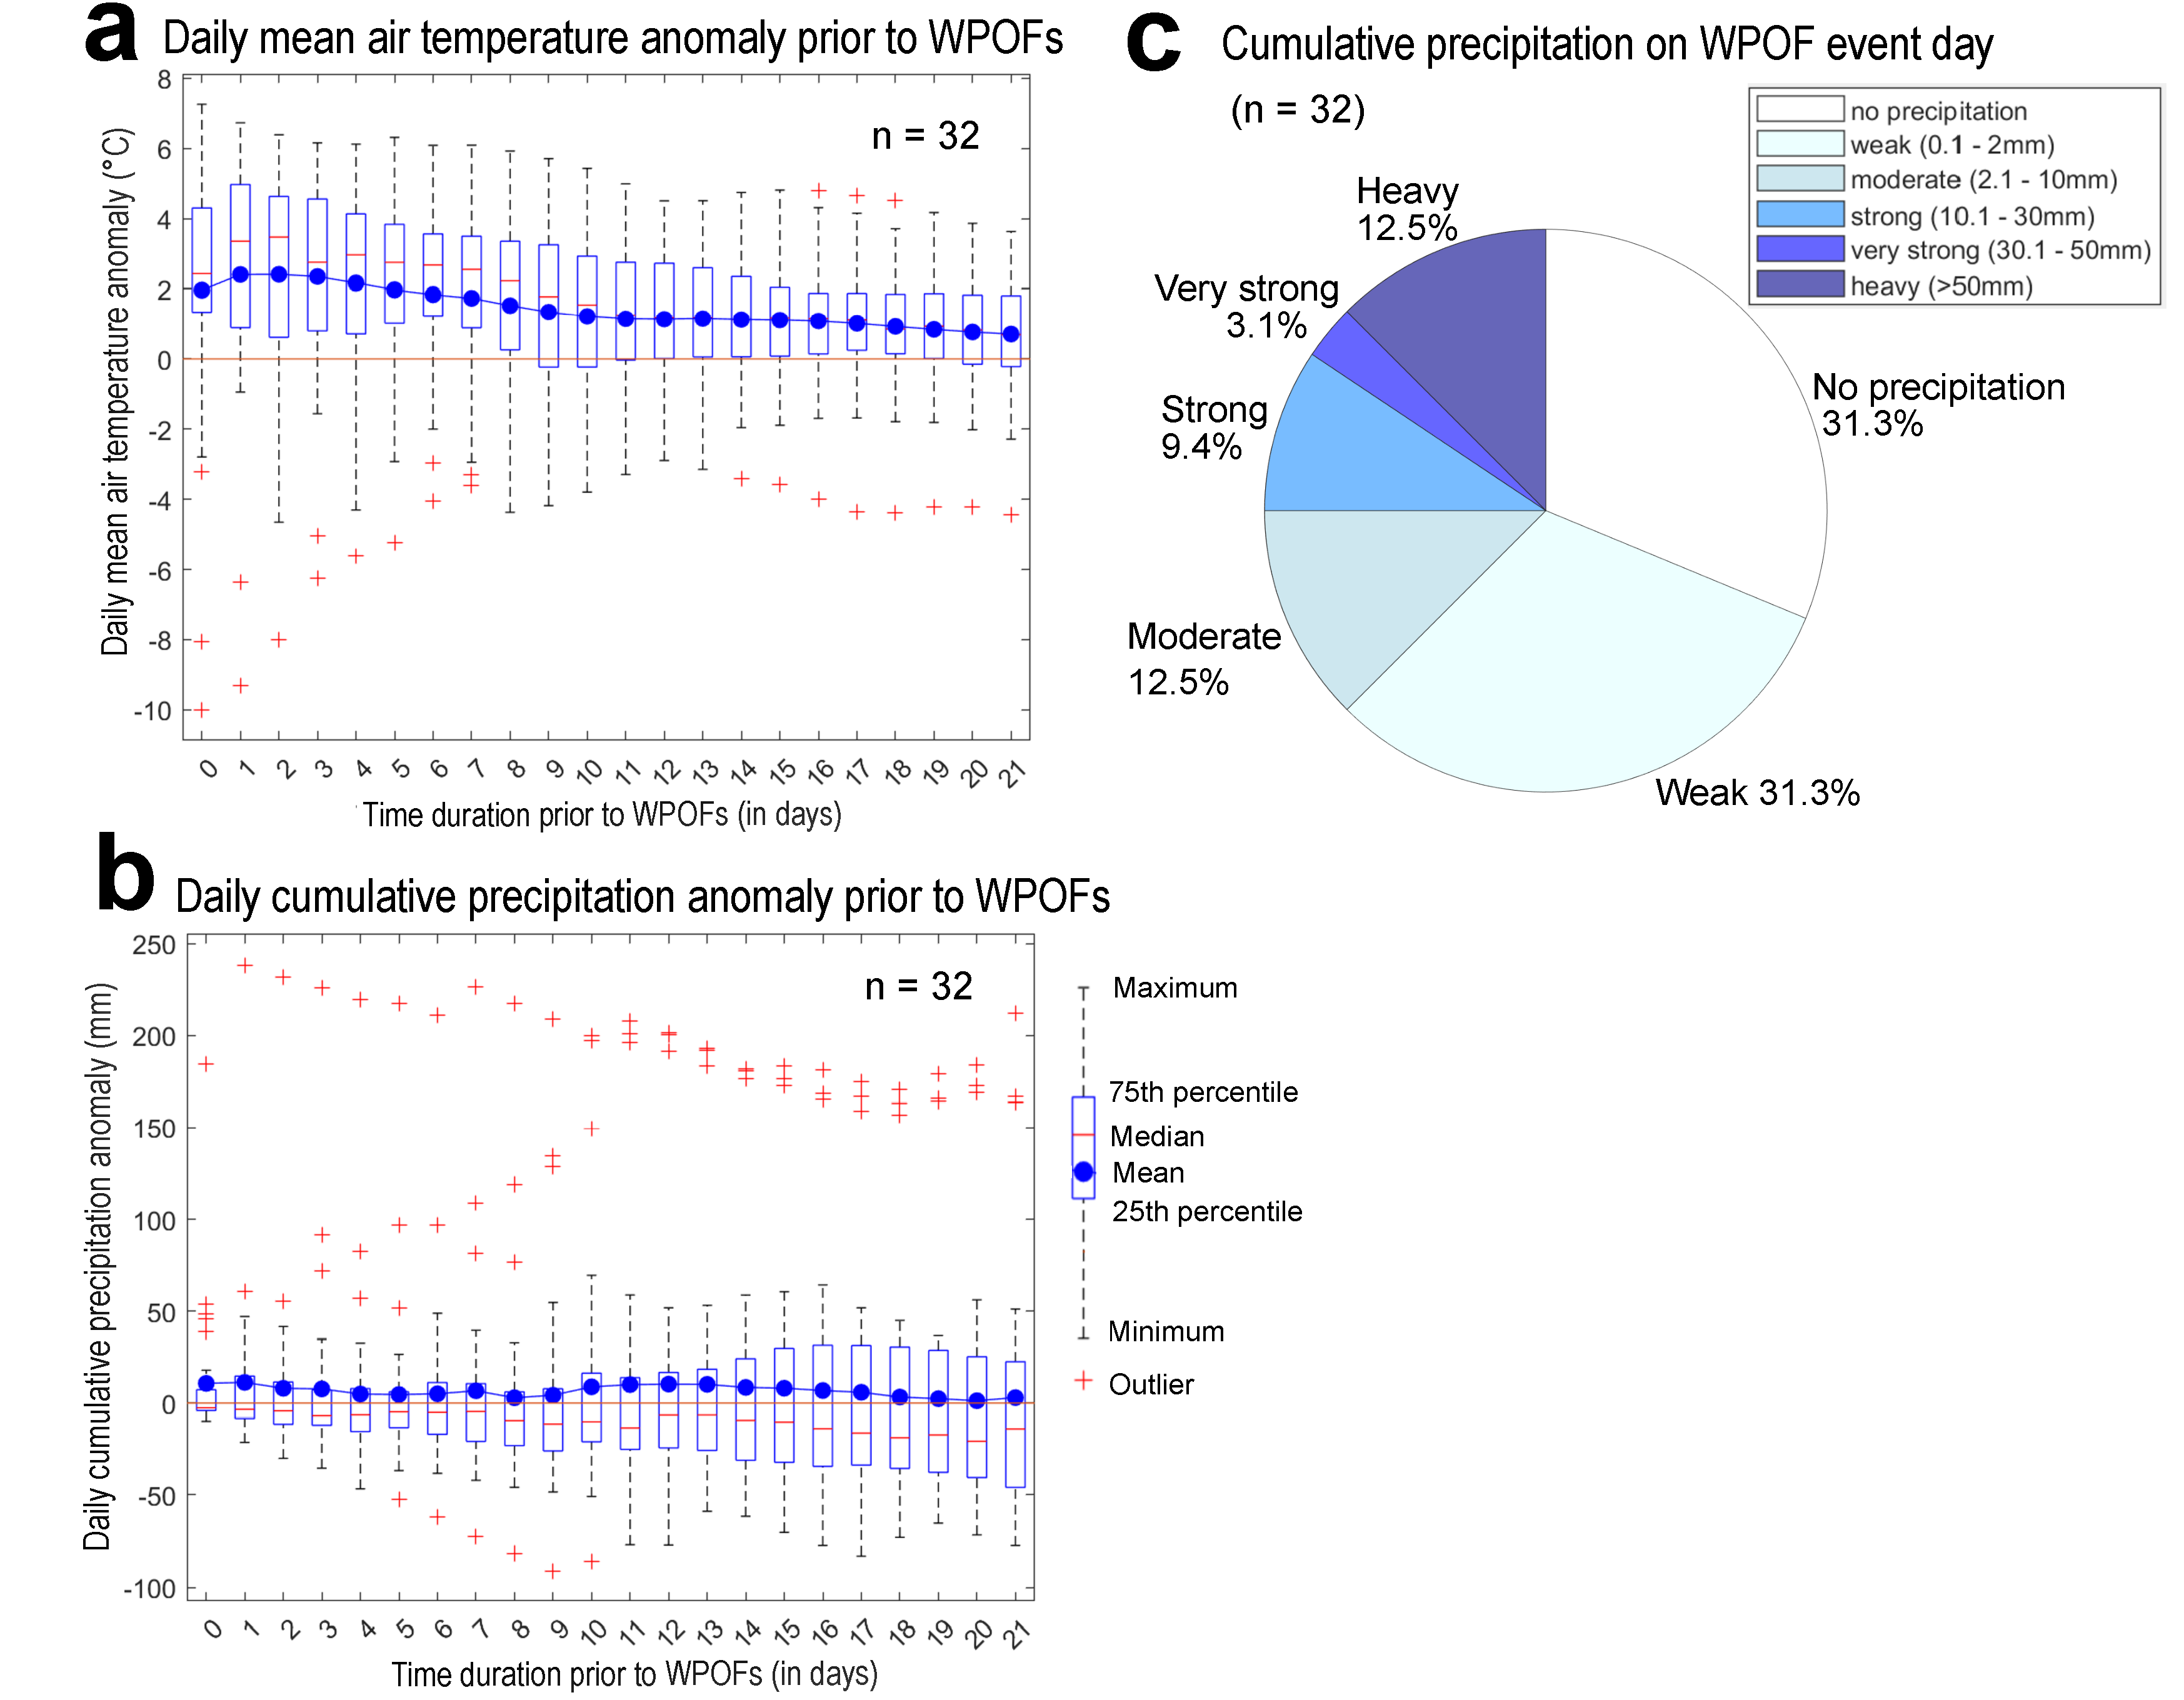
\includegraphics[width=1\linewidth]{chapters/chapter_WPOFs/meteo_anomaly.pdf}
    \caption{Meteorological conditions prior and during documented WPOFs in the Swiss Alps since 1961 with exactly known event dates (n = 32). a) Daily mean air temperature anomaly and b) cumulative precipitation anomaly for 0 to 21 days prior to WPOFs. For both panels, the mean (blue dot), the median (red dash), the 75$^{th}$ and the 25$^{th}$ percentile are shown. The red crosses represent outliers that are more than 1.5 times the interquartile range away from the bottom or top of the box (the interquantile range is the distance between the bottom and top of each box). c) Cumulative precipitation over WPOF glaciers on the event day, classified into six categories (from no precipitation to heavy precipitation) according to MeteoSwiss thresholds.}
    \label{fig:mto_anomaly}
\end{figure*}


\subsection{ Glacio-geomorphic characteristics of WPOF glaciers}
\label{sec:envelop_geo}

Figure~\ref{fig:distribution_geo} shows the accumulation area ratio, relative coverage with supraglacial debris, the glacier's average slope, mean aspect, surface area, median elevation, and mean ice surface velocity, for both Swiss glaciers with at least one reported WPOF and for all glaciers in Switzerland. The results show that (i) the median area of glaciers with reported WPOF events is thirty times larger than the median area of all Swiss glaciers (2.72\,km$^2$ vs. 0.09\,km$^2$), (ii) the average ice surface velocity is 2.5 times higher for glaciers with WPOFs than it is for the other glaciers (12.88 vs. 4.98\,m\,yr$^{-1}$), and iii) the median of the average slope is 11° less steep for glaciers with reported WPOFs compared to all other glaciers (28.2°). We conducted Mann-Whitney U tests to assess the significance of the differences between the statistical distribution of glacio-geomorphic variables of glaciers with and without reported WPOFs. Our findings revealed that all variables, except aspect, exhibited statistically significant differences at the 0.05 level. However, we question the interpretability of this significance for two reasons. First, the observations could potentially be influenced by observational biases, as larger WPOFs from larger glaciers might be more often recognized and reported than those from smaller glaciers. Second, the number of glaciers with known WPOFs (n=37) may be too small compared to the entire glacier population in Switzerland (n=1400) to draw robust conclusions. We conclude that, based on our dataset, there is no obvious set of glacier-wide glacio-geomorphic variables that would allow distinguishing between glaciers that are prone to WPOFs and glaciers for which WPOFs are unlikely to occur. This result aligns with \citet{Haeberli1983}, and we suggest that the occurrence of WPOFs is likely controlled by smaller-scale topographic or glacio-geomorphic features, for which there is too little information in the analysed variables evaluated at the glacier-wide scale. Most importantly, there is no information on the exact location of the water pockets for most cases, which prevents a smaller-scale analysis.  


\begin{figure*}
    \centering
    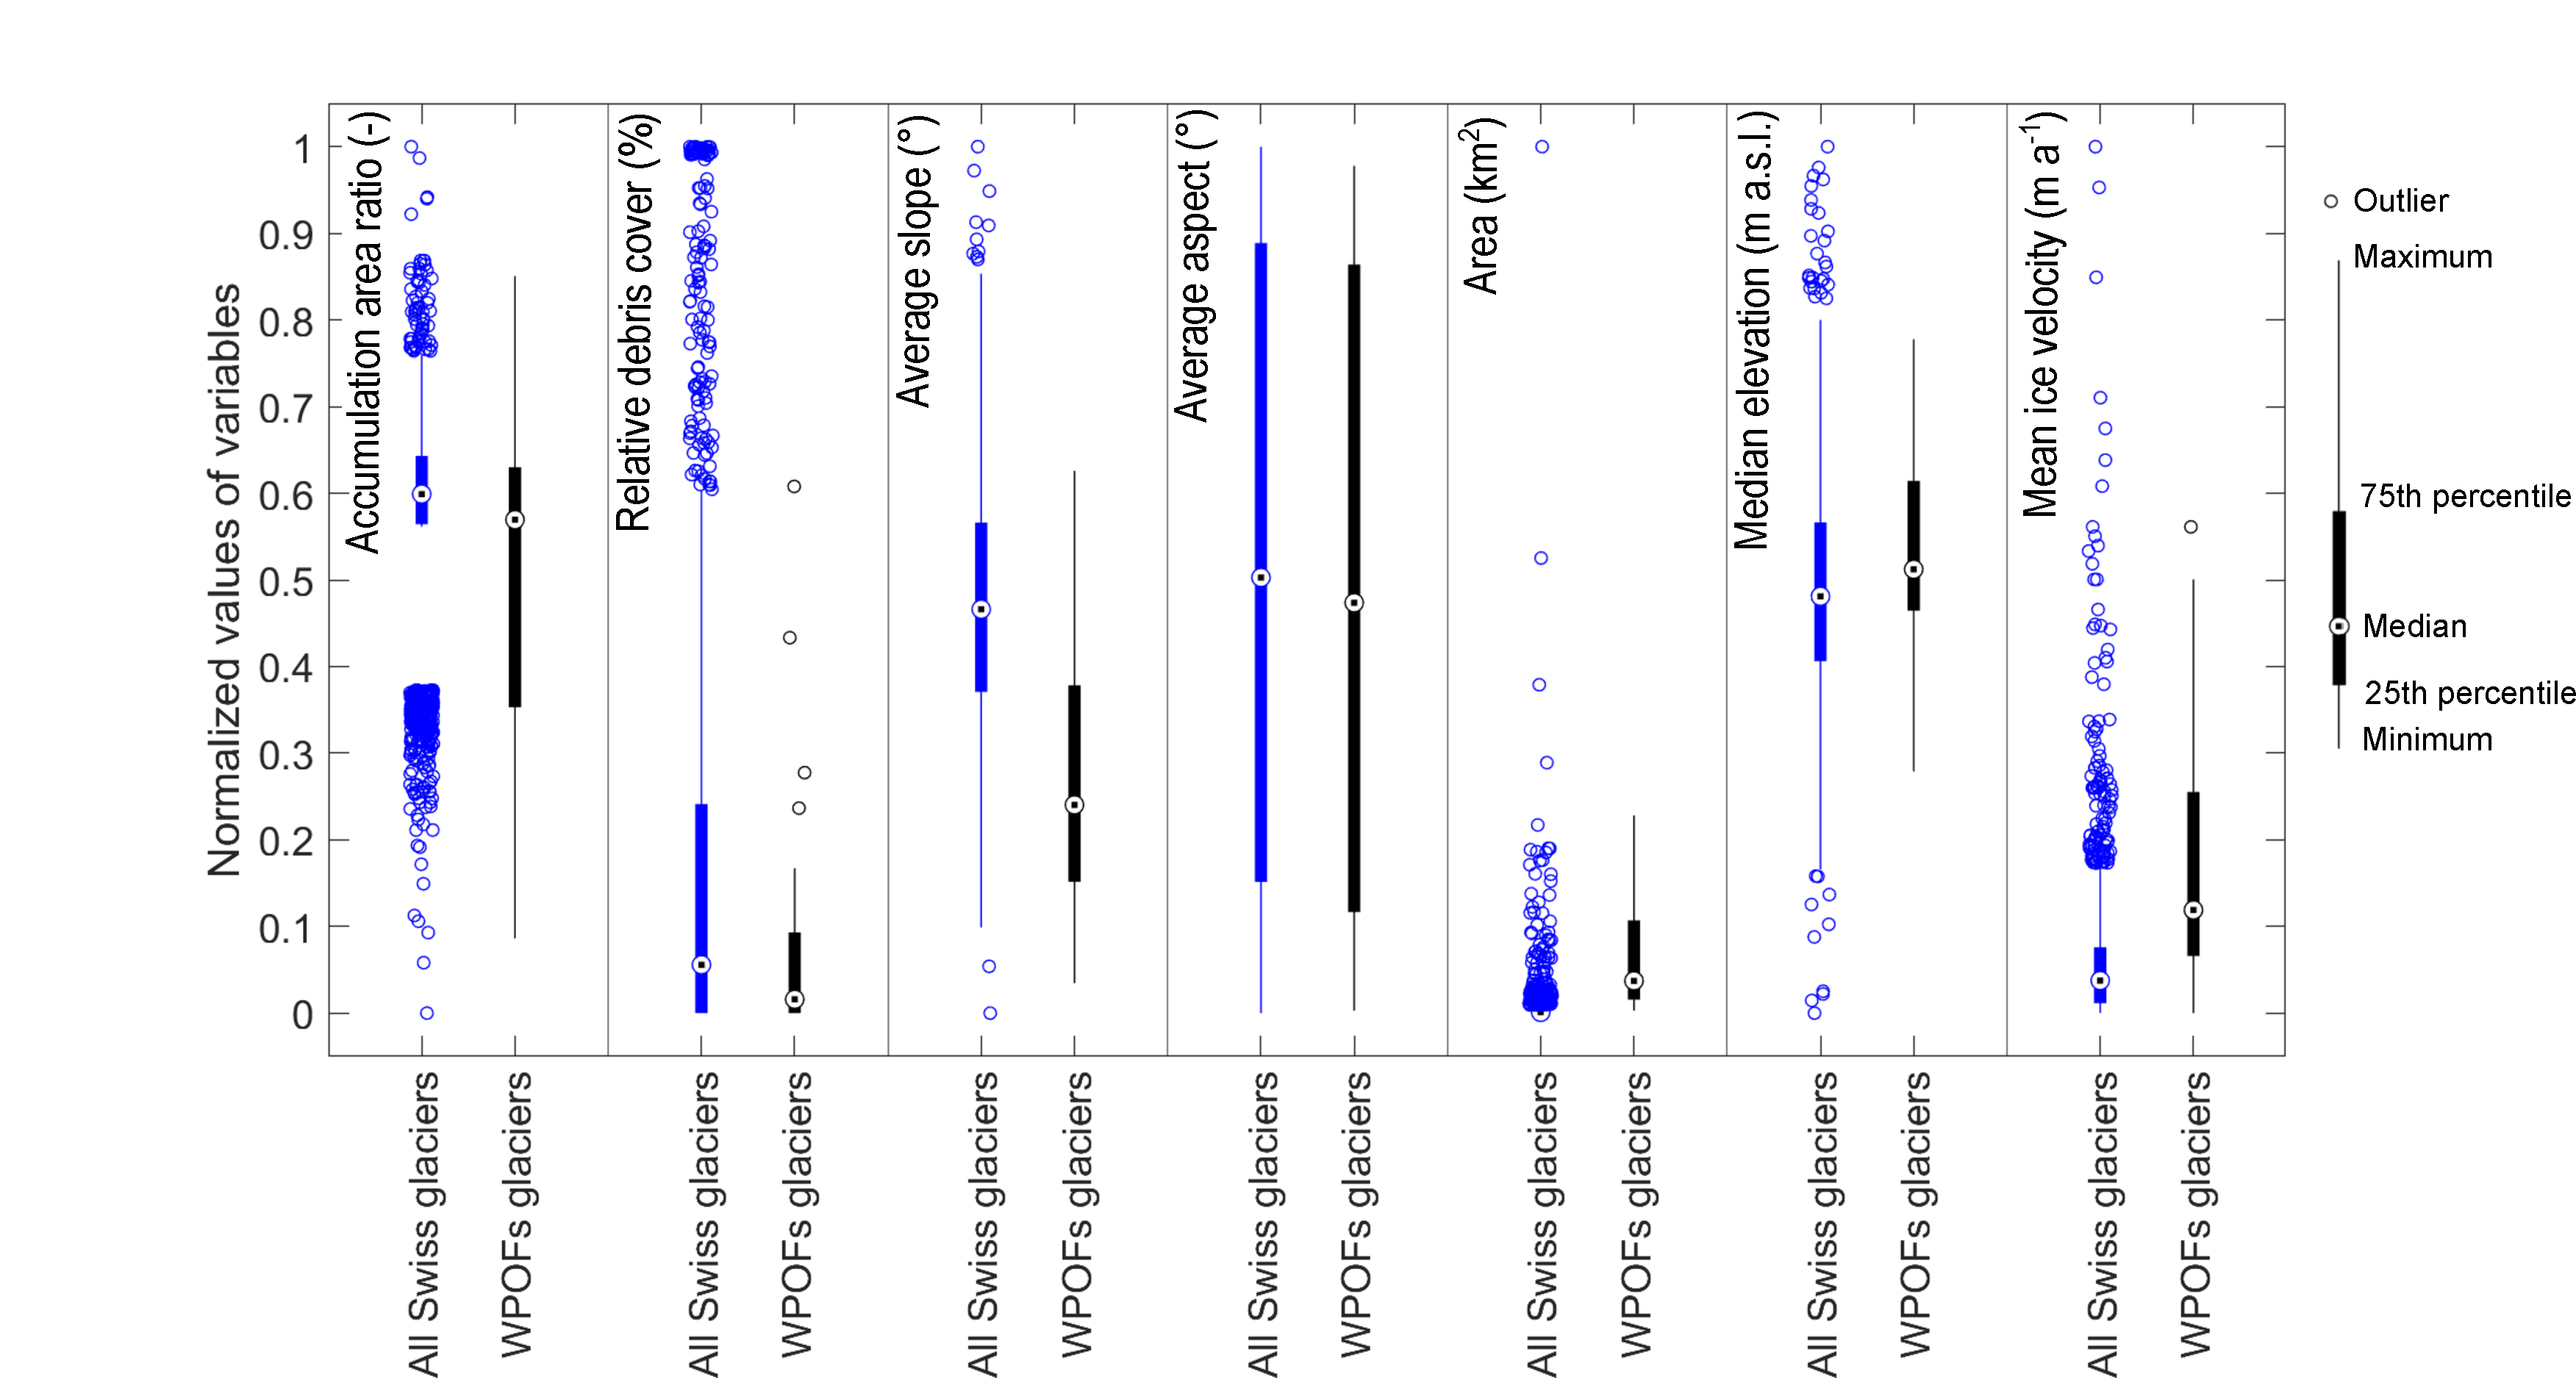
\includegraphics[width=1\linewidth]{chapters/chapter_WPOFs/geomorpho_variables.pdf}
    \caption{Distribution of glacier-wide glacio-geomorphic variables for Swiss glaciers with reported WPOFs (n = 37, in black) based on the temporally closest  Swiss glacier inventory \citep{Muller&al1976, Maisch&al2000, Linsbauer&al2021} as well as data from \cite{Altrock2022} and \cite{Millan&al2022}, and for all glaciers in Switzerland (in blue) based on the latest Swiss glacier inventory (SGI2016, \citet{Linsbauer&al2021}). Variables values are normalized. The median (circle with dot) and the interquartile range (box) are shown for each variable. The unfilled circles represent outliers that are more than 1.5 times the interquartile range away from the bottom or top of the box.}
    \label{fig:distribution_geo}
\end{figure*}




\section{ Hypotheses for the formation of glacial water pockets and their outbursts mechanisms}
\label{sec:mechanisms}

Based on the updated WPOF inventory for the Swiss Alps and a literature review, we propose four mechanisms describing the formation of water pockets in alpine glaciers. These formation mechanisms comprise all the processes involved in the evolution of the water pocket, from its growth and filling to its eventual rupture. In our inventory, we identified a total of 16 WPOFs for which available event descriptions help to understand the formation mechanisms. The documented formation mechanisms can be divided into the following three categories: 1) temporary blockage of subglacial channels (10 WPOFs), 2) hydraulic barrier (5 WPOFs), and 3) water-filled crevasses (1 WPOF). The mechanism of formation for the remaining 75 events remains unknown. In addition, we present a fourth formation mechanism that hasn't been described for any WPOF in the Swiss inventory but that is well known and described in literature from the case study of Glacier de Tête Rousse in the French Alps \citep{Vincent&al2010b}: 4) thermal barrier. Figure~\ref{fig:general_concept} schematically shows the four water pocket formation mechanisms we propose. 



\begin{figure*}
    \centering
    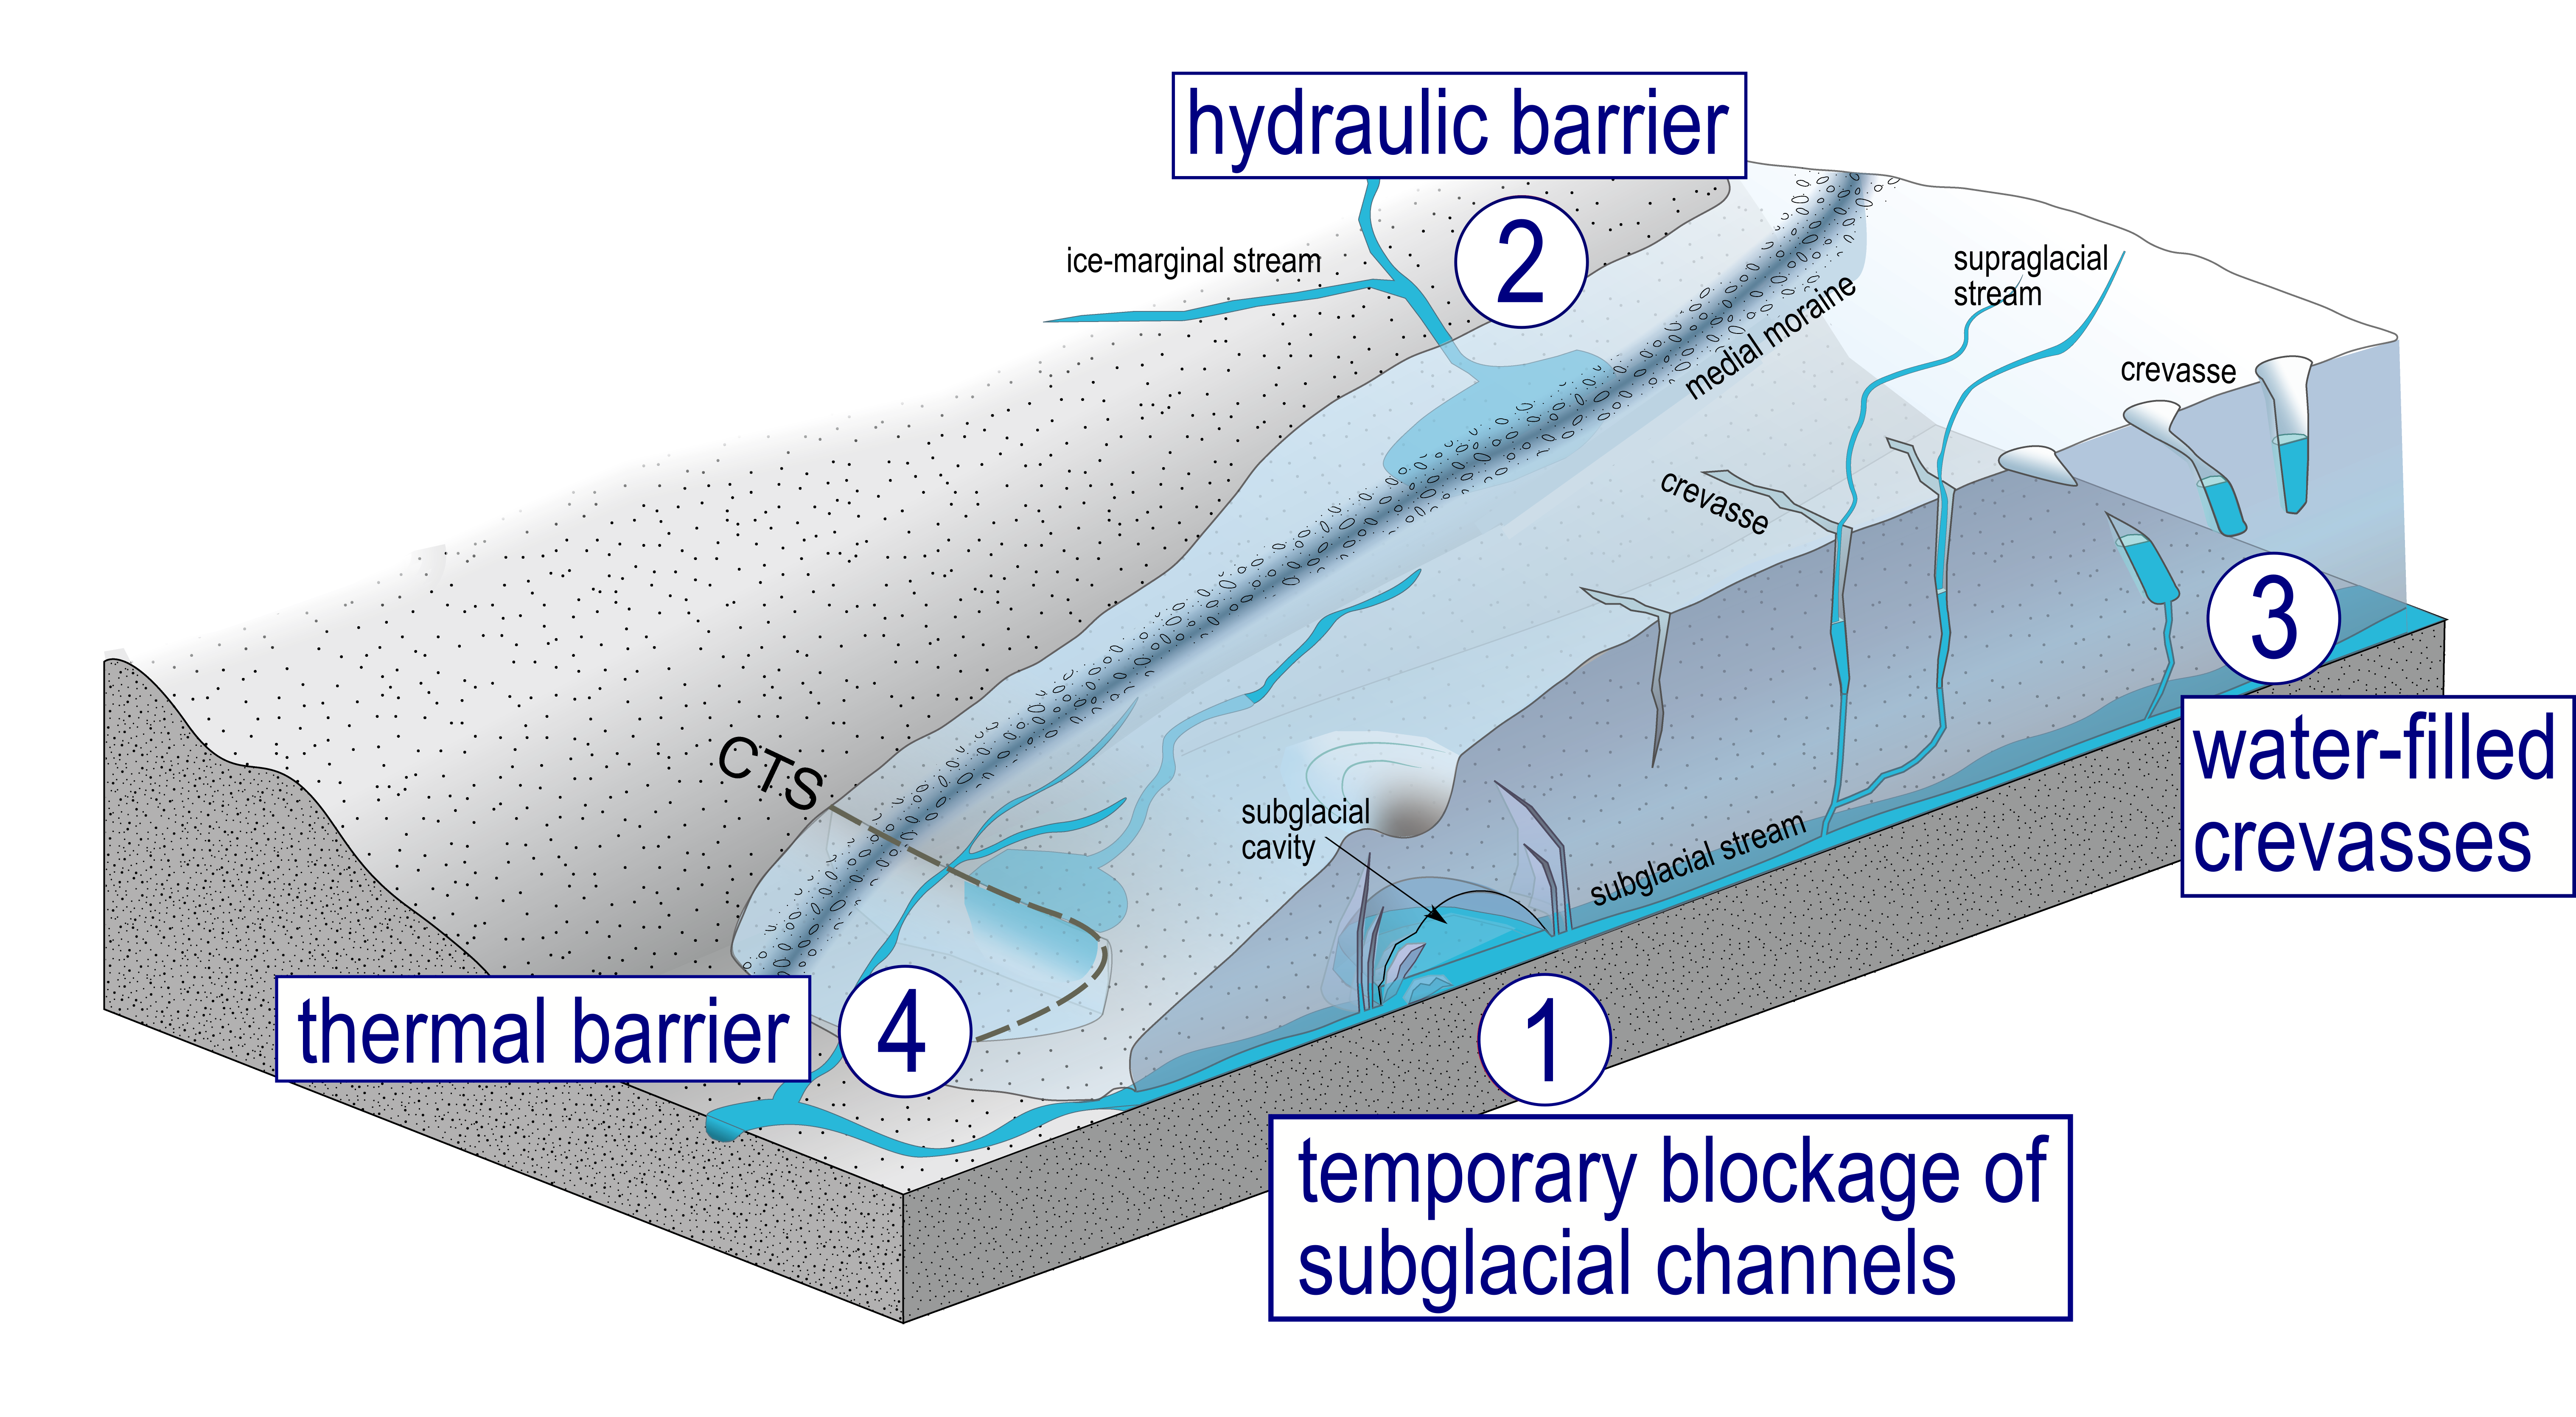
\includegraphics[width=0.75\textwidth]{chapters/chapter_WPOFs/ReviewMechanisms.png}
    \caption{Schematic representation of the proposed four main mechanisms of water pocket formation in alpine glaciers: 1) temporary blockage of subglacial channels, 2) hydraulic barrier, 3) water-filled crevasses, and 4) thermal barrier. CTS indicates the cold-temperate transition surface, i.e.\ the surface along which the ice of a polythermal glacier transitions from cold to temperate.}
    \label{fig:general_concept}
\end{figure*}


\subsection{ Temporary blockage of subglacial channels}
\label{sec:subglacialblocking}


Temporary blockage of subglacial channels by ice blocks collapsing from the channel roof has the potential to accumulate water within the glacier, which can be released suddenly when the temporary ice dam breaks \citep{Ballantyne&McGann1980,Rounce&al2017,Swift&al2021}. Typical summer discharges of proglacial melt water streams for medium-sized alpine glaciers can easily be in the order of 10\,m$^3$\,s$^{-1}$ \citep{Werder&al2010,Muller&al2024}. Thus, it would only take a few hours to accumulate a water reservoir of a few thousands of m$^3$ in a blocked subglacial channel. This mechanism is illustrated in Figure~\ref{fig:IceBlockage}a. Note that for the roof collapse to occur, the subglacial channel needs to have temporarily free-surface flow.

According to event descriptions and information stored in our inventory, temporary blockage of subglacial channels was observed at Rhonegletscher in 1900, 1934 and 1947, at Findelgletscher in 1943 and 2017, at Hubelgletscher in 2004, at Oberer Grindelwaldgletscher in 2011, and at Griesgletscher in 2023. In terms of the size of events related to this formation mechanism, information is only available for three cases. At Findelgletscher on August 4th 2017, the estimated total flood volume was 17'000\,m$^3$ (hourly-gauged, baseflow excluded), and the maximal hourly discharge measured 1.5\,km downstream of the glacier portal was 15\,m$^3$\,s$^{-1}$ (which is four times larger than the baseflow, see Fig.~\ref{fig:IceBlockage}b). At Oberer Grindelwaldgletscher in 2011, the total estimated flood volume between August 25th and 27th was 300'000\,m$^3$ (4\,min-gauged, three-days average baseflow excluded \citep{Hahlen2011}), and the maximal discharge measured 4\,km downstream of the glacier portal was 73\,m$^3$\,s$^{-1}$ on August 25th (which is five times larger than the baseflow, see Fig.~\ref{fig:IceBlockage}c). At Hubelgletscher in 2004, the estimated total flood volume on August 4th was 21'500\,m$^3$ (10\,min-gauged, baseflow excluded), and the maximal hourly discharge measured 15\,km downstream of the glacier portal was 22\,m$^3$\,s$^{-1}$ (which is 147\,\% of the baseflow, see Fig.~\ref{fig:IceBlockage}d). After the event, the empty englacial cavity volume (see Fig.~\ref{fig:WPOFs_evidences}) was estimated to 2100\,m$^3$ by \cite{fink2004}. 

We hypothesise that the collapse of ice blocks that can form an ice dam is more likely within subglacial cavities than within regular subglacial channels (i.e. R-channels described in \cite{Roethlisberger1972}), and that the potential storage volume is correspondingly larger in cavities. Here, we refer to "subglacial cavity" for voids that are significantly bigger than the so-called linked subglacial cavities that are part of an inefficient subglacial drainage system \citep[e.g. Fig. 14 in][]{Fountain&Walder1998}. Partial collapse of the roof is more likely to occur in a subglacial cavity because its geometry is driven by the failure of an ice roof consisting of ice lamellas \citep{Ogier&al2022, Rass&al2023}. Collapsing ice lamellas are necessary to suddenly and temporarily block the free-surface streamflow in subglacial cavities, whereas the geometry of regular subglacial channels is more controlled by the interplay between ice melt at the water-ice interface vs. ice creep \citep{Roethlisberger1972}.

In thin ice, the partial collapse of a cavity's roof can be observed at the glacier surface through the presence of circular crevasses centred around the cavity. The collapse of ice blocks is frequent during the development of subglacial cavities above subglacial channels \citep{Egli&al2021, Ogier&al2022}. The development of circular crevasses soon after a WPOF (i.e. stage 4 in Fig.~\ref{fig:IceBlockage}a) was observed at Hubelgletscher in 2004 (see Fig.~\ref{fig:WPOFs_evidences}) and at Findelgletscher in 2017 .  

The fact that the temporary blockage of subglacial channels is a plausible water pocket formation mechanism is also supported by the presence of ice blocks in the proglacial stream during the outburst, and by a cut-off of the stream discharge before the outburst \citep[as described in][]{Ballantyne&McGann1980}. Floating blocks of recently collapsed ice were observed in the proglacial stream of Findelgletscher in 2017 \citep{Swift&al2021}, and at Griesgletscher in 2023 (see Fig.~\ref{fig:WPOFs_evidences}). Discharge cut-off before a WPOF was observed at Rhonegletscher in 1934 and 1947 \citep{Mercanton1948}, at Oberer Grindelwaldgletscher in 2011, and at Findelgletscher in 2017 (see Fig.~\ref{fig:IceBlockage}b and c). The sharp increase in discharge at Findelgletscher (Fig.~\ref{fig:IceBlockage}b) is in line with a sudden breaching of the ice dam (see \cite{Haeberli1983}). For Hubelgletscher in 2004, the hydrograph of the WPOF exhibits a sharp peak, likely due to an abrupt ice dam rupture \citep{fink2004}. However, the distant gauging station fails to capture a discharge cut-off signal (Fig.~\ref{fig:IceBlockage}d), possibly because of the relatively high meltwater contributions from other glaciers to the flow signal compared to the two previous cases. For all examples in Figure~\ref{fig:IceBlockage}, the life time of the natural dam temporarily blocking subglacial drainage that is shown by the discharge cut-off duration was relatively short (a few minutes (Fig.~\ref{fig:IceBlockage}c) to a few hours (Fig.~\ref{fig:IceBlockage}b)). 

In the Alps, the formation of circular crevasses associated to subglacial cavities is increasing with rising air temperature \citep{Stocker&al2017,Egli&al2021}. So far, however, it remains unclear whether WPOFs caused by temporary blockage of subglacial channels are occurring more often because of atmospheric warming. This is because no clear trend in the frequency of documented WPOFs was observed in past decades (Fig.~\ref{fig:WPOFs_map}b), and the specific mechanisms behind these occurrences are also not well-documented.

\begin{figure*}
    \centering
    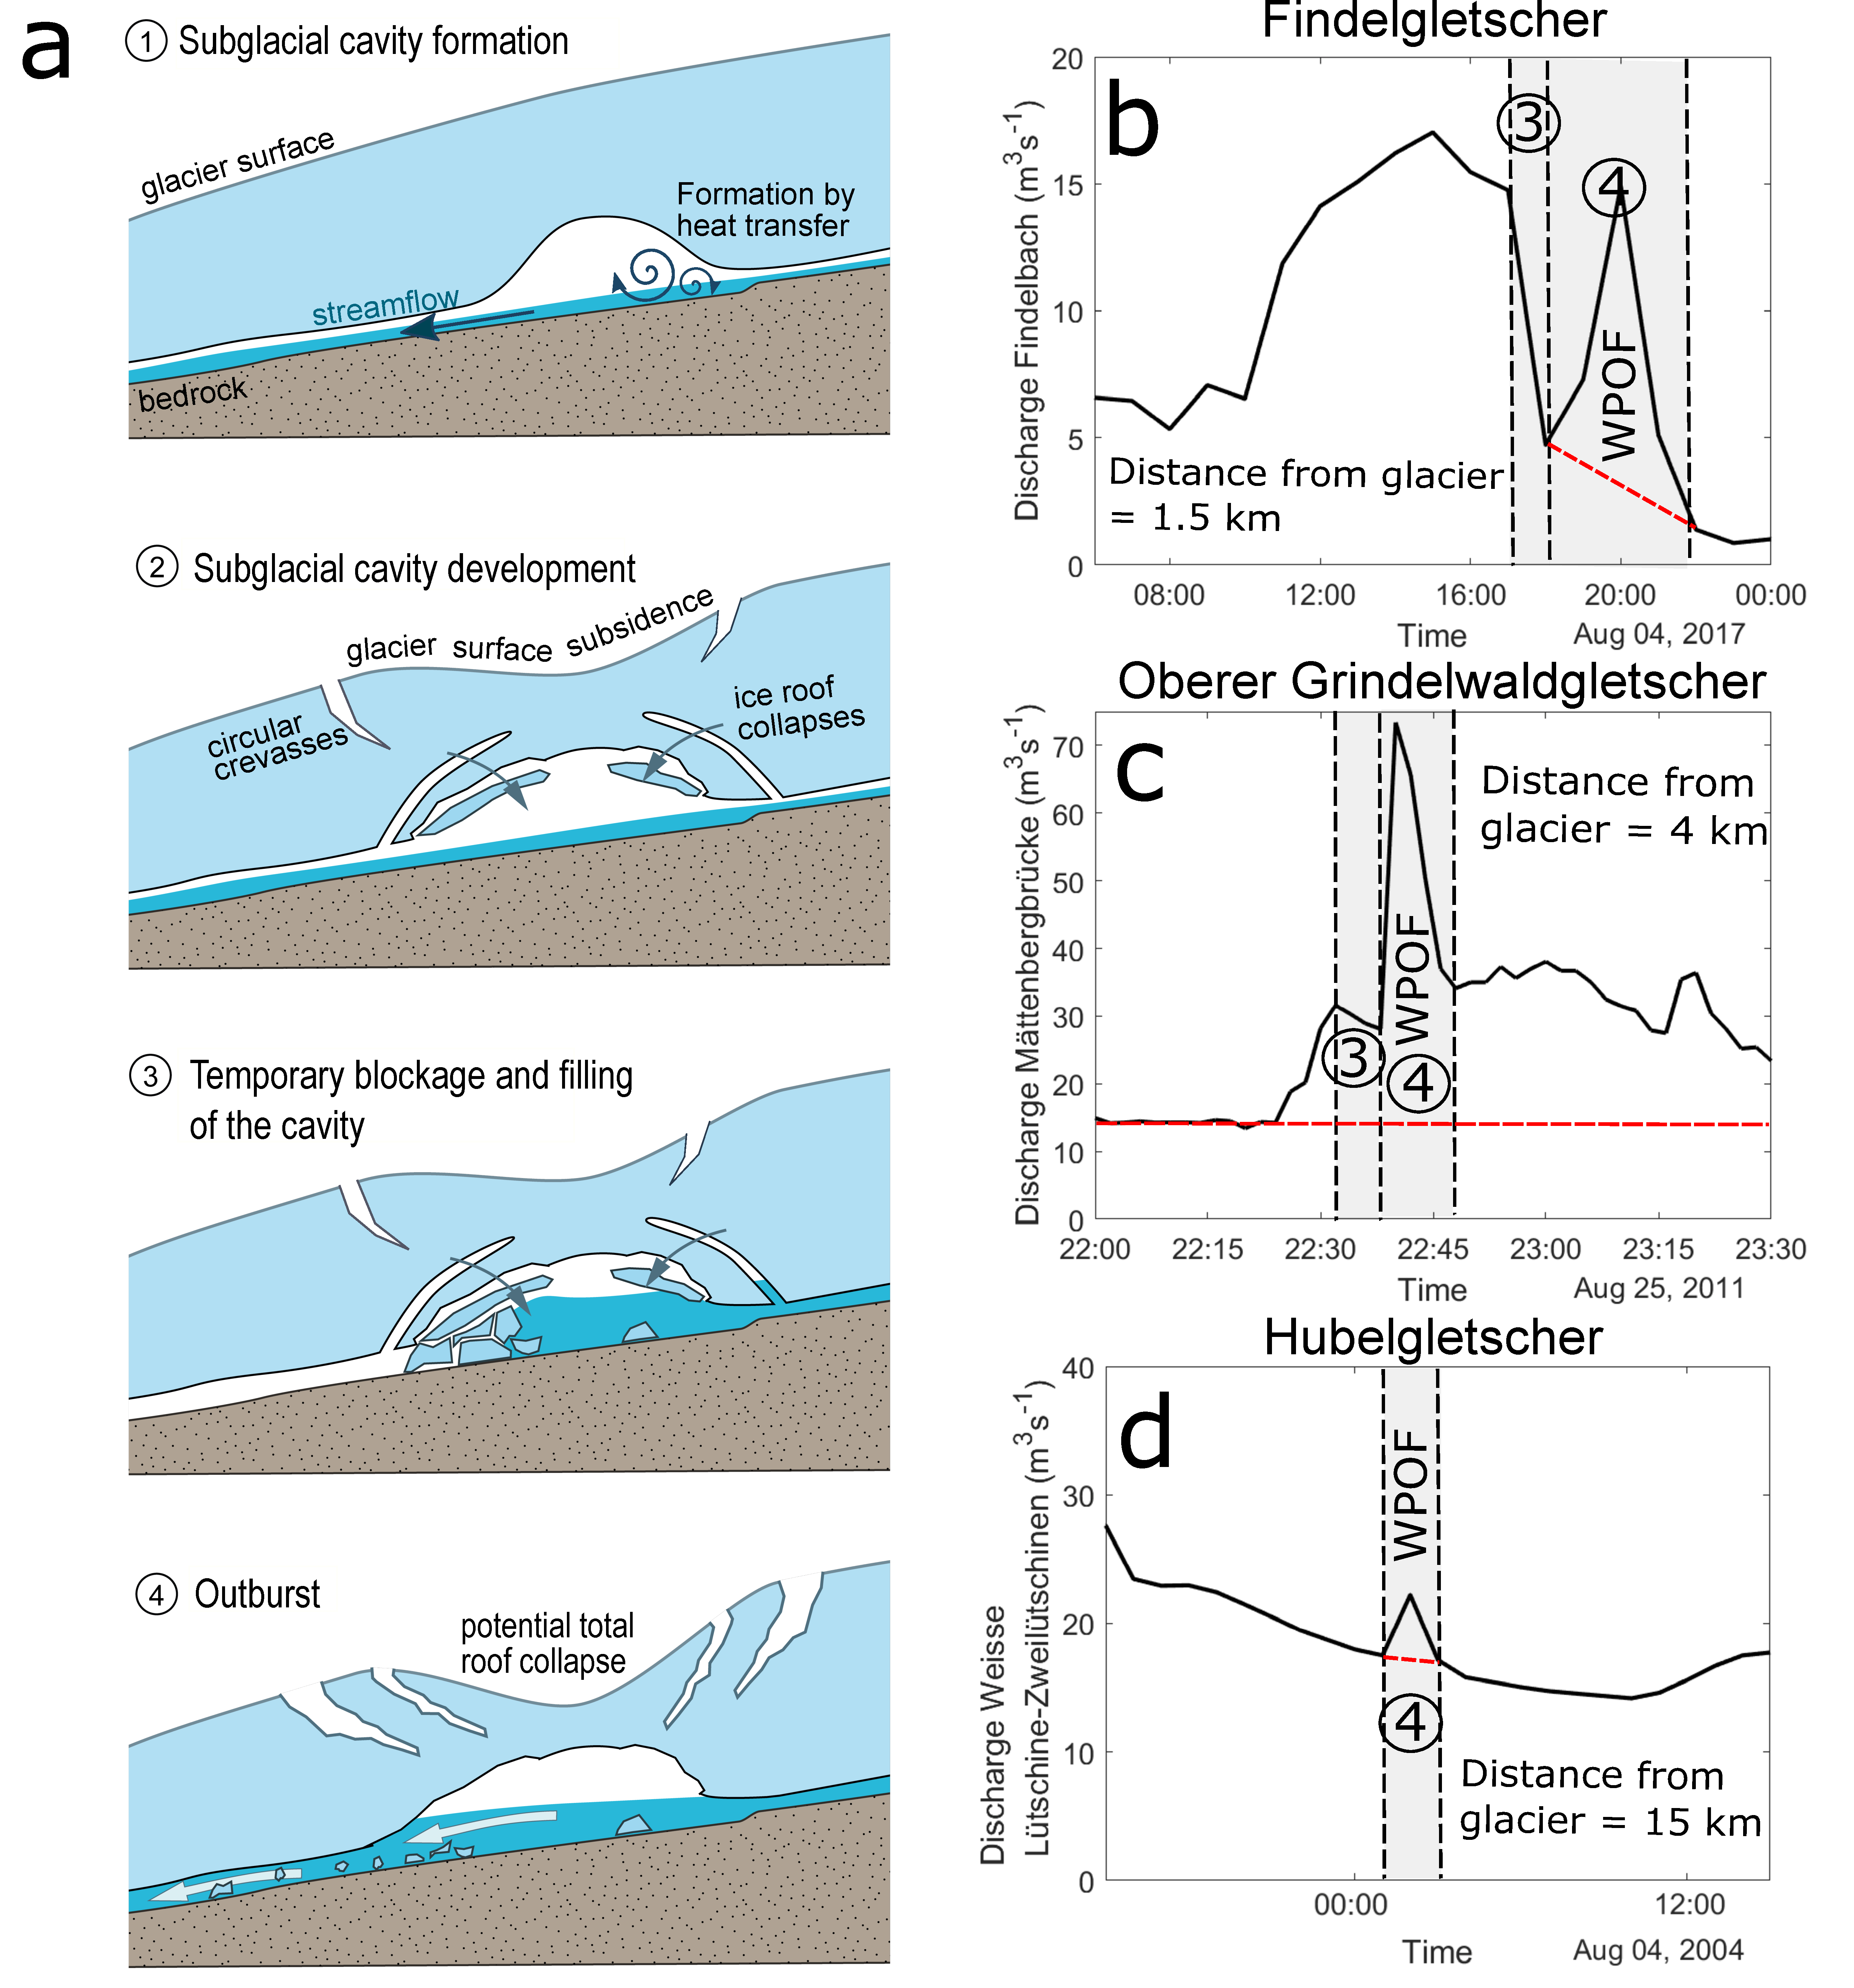
\includegraphics[width=1\textwidth]{chapters/chapter_WPOFs/Temp_blockage.pdf}
    \caption{ WPOFs originating from temporary blockage of subglacial channels. a) Schematic development of temporary blockage of subglacial channels, linked to the potential collapse of subglacial cavities. b)-d) Examples of hydrographs for three WPOFs in the Swiss Alps for which a temporary blockage of the subglacial channel is assumed to have caused the WPOF. Note the different scales for both the x- and y-axes in the three panels. The shaded areas separated by dashed lines and the numbering represent different phases of WPOF events and correspond to the numbers in a): 3) drainage cut-off linked to subglacial blockage and cavity filling, and 4) sudden, fast and sharp increase followed by fast decrease in discharge, linked to the outburst flood caused by sudden break (mechanical breach) of the subglacial ice dam. The estimated baseflows to calculate the flood volumes are indicated by the red dashed lines.}
    \label{fig:IceBlockage}
\end{figure*}


\subsection{ Hydraulic barrier}
\label{sec:hydraulic_barrier}

Water accumulates at the glacier bed in areas with a local minimum in the hydraulic potential. The ice surrounding these areas of low hydraulic potential can act as hydraulic barriers for the subglacial water flow, and we hypothesise that these hydraulic barriers constrain potential locations for the formation of water pockets. To understand where these hydraulic barriers form, we write the subglacial hydraulic potential $\psi$ in meters water-equivalent (i.e.\ the hydraulic head) as

\begin{equation}
     \psi = \frac{p}{\rho_w\,g} + z_b,
     \label{eq:phi1}
\end{equation}
%
where $p$ is the water pressure, $g$ the gravitational acceleration, $\rho_w$ the density of water and $z_b$ the elevation of the bedrock \citep{Cuffey&Paterson2010}. \cite{Shreve1972} assumed that water pressure is equal to the overburden ice pressure, and thus
%
\begin{equation}
     \psi_S = \frac{\rho_i}{\rho_w}\,(z_s - z_b) + z_b = \frac{\rho_i}{\rho_w}\left(z_s + z_b\,\left(\frac{\rho_w}{\rho_i} - 1\right)\right) \approx \psi,
     \label{eq:p1}
\end{equation}
%
where $\rho_i$ and $\rho_w$ are the ice and water density, respectively, and $z_s$ is the glacier surface elevation. 

Figure~\ref{fig:plainemorteWP}a shows the conceptual case of a water pocket formed by a hydraulic barrier, with the hydraulic head $\psi_S$ defined in Equation~\ref{eq:p1}. Note that this case example is computed by using real data presented in Figure~\ref{fig:plainemorteWP}b and described later in this section. The hydraulic barrier at the seal is caused by a rise in surface elevation along the general direction of englacial and subglacial water flow (note that in Equation~\ref{eq:p1}, $\psi_S (seal)$ is mainly sensitive to surface elevation since $\rho_w/\rho_i - 1 \approx 0.09$). The maximum water pocket extent is controlled by the highest point of the hydrauic head situated at the hydraulic barrier (the seal) which in turn sets the height the water pocket can reach on the opposite shore $z_A$. Thus, the maximal hydraulic head which can be reached within the water pocket ($z_A + (\rho_i/\rho_w) h_A$) is the head at the seal ($h_A$ being the ice thickness at point $A$). Once that head is exceeded, the barrier brakes. As long as there is water input for the pocket to grow and the water within the pocket does not reach point $A$, the water pocket accommodates the new water by lifting the overlaying ice (see Appendix~\ref{Appendix:subglacialWP} for water pocket depth and volume calculation).

In Figure~\ref{fig:plainemorteWP}a, the water pocket is at the rupture point as the water pocket extent reaches the point $A$, i.e.\ the point where the hydraulic head within the pocket equals the head at the seal. At this point, the seal breaks by ice dam flotation and the reservoir empties through a sheet flow and eventually by channel enlargement \citep[this is similar to ice-marginal and subglacial lakes outburst floods mechanisms, see][]{Bjornsson2010}. Note that in Fig.~\ref{fig:plainemorteWP}a, the hydraulic head at $A$ is higher than the glacier surface at the minimum hydraulic head, which means that if there is a hydraulic connection between the surface and the water pocket, then a pond could form at the surface before the outburst. However, if there is no hydraulic connection, then the ice roof of the water pocket can lift up during the filling phase and this should be visible from the surface. During the drainage phase, one should be able to observe the surface to lower and potentially the appearance of circular crevasses \citep[e.g.][]{Konrad1998}. After an outburst, local minima of hydraulic head, driven by glacier surface and bedrock topography, can still remain. This could explain the repetitive occurrence of WPOFs for some of the glaciers in our inventory with multiple documented events. 

The hydrograph of an outburst caused by the break of an ice-dammed lake (for which we assume the same rupture mechanism as presented here) can show either a sudden rise in discharge (in less than an hour) followed by a slow decrease in discharge, or a slow rise in discharge (over hours to days) followed by a sudden decrease in discharge \citep[see schematic hydrographs of Fig. 4 in][]{Roberts2005}. This latter case implies that, to be detectable, outbursts of this type would need to originate from water pockets located relatively close to the glacier portal. For water pocket ruptures of this type located further up the glacier, the flood hydrograph would be buffered by the travel through the subglacial drainage network, making such a water pocket rupture hard to detect. 

The WPOFs at Glacier d'Orny in 1920 and Minstigergletscher in 2008 are suspected to have been caused by a hydraulic barrier, similar as shown in Fig.~\ref{fig:plainemorteWP}a. At Glacier d'Orny, \cite{Mercanton1921} suggested that the previous glacier advance modified the subglacial topography at the glacier tongue, creating an ice dam for the subglacial streamflow until the water pressure exceeded the dam's resistance. At Minstigergletscher (see Fig.~\ref{fig:WPOFs_evidences}), the presence of debris at the glacier surface led to differential surface melt, locally thicker ice and, in turn, to a hydraulic barrier, i.e.\  steep gradients and a local depression in the hydraulic potential field . The water pocket was likely formed through the filling of existing subglacial voids near the location of the hydraulic barrier. \cite{Konrad1998} also explained a possible water pocket formation at Mendel Glacier in the Sierra Nevada (California) by a local minimum in the hydraulic potential right below a topographic depression at the glacier surface (see her conceptual Fig.~9). The author hypothesised that the depression formed because of differential ice melt at the ice-debris boundaries, similar to the Minstigergletscher case discussed above. 

Due to the typical nature of the en-/subglacial drainage system in alpine glaciers, a hydraulic barrier alone is not a sufficient requirement for a water pocket to form. For instance, if there is an existing englacial conduit that links the water reservoir located at the hydraulic barrier to the glacier surface, the extra water pressure may not lift the ice to form a water pocket but instead lead to the formation of a pond at the surface. Taken together, this means that a hydraulic barrier may not be impermeable enough to seal the upstream area sufficiently; in fact, this is probably the case at most such locations.

To analyse the potential presence of hydraulic barriers in Swiss glaciers, we mapped theoretical hydraulic barriers. We used the open-source package \textit{WhereTheWaterFlows.jl} (see Supplementary Materials). The necessary input data to map the distributed hydraulic potential with this tool are glacier surface and bedrock topography. We used surface and bedrock digital elevation models (DEMs) for all glaciers in Switzerland with a spatial resolution of 10\,m and source dates from 2013 to 2018 \citep{Grab&al2021}. The tool does not account for temporal fluctuations in water pressure and is limited by the spatial resolution of the DEMs used. As a consequence, only relatively large potential subglacial water pockets sealed according to the hydraulic barrier mechanism are indicated by our approach, and small water pockets caused by local-scale topographic features (e.g. the water pocket at Minstigergletscher described above) cannot be resolved. For 17 out of the 37 glaciers with known WPOF events (i.e.\ 46\,\%), our analysis identified current locations where water is likely to accumulate by a hydraulic barrier. Note that this result cannot be related to past events (i.e.\ before 2013) because we calculated the hydraulic potential with data on the present glacier extents and surface topography. Interestingly, out of the 1400 glaciers we examined, our analysis identified hydraulic barriers in only 93 of them (i.e.\ 6\,\%).  Fig.~\ref{fig:plainemorteWP} shows an example of a possible water pocket formation by a hydraulic barrier at Glacier de la Plaine Morte (Switzerland): the water pocket would form at the local minimum of the Shreve hydraulic potential (Fig.~\ref{fig:plainemorteWP}b), which can be explained by the local depression at the glacier surface (Fig.~\ref{fig:plainemorteWP}a). We note that even though this glacier experienced lake outbursts on a regular basis \citep{Lindner&al2020,Ogier&al2021}, no WPOF was ever reported.


\begin{figure*}
    \centering
    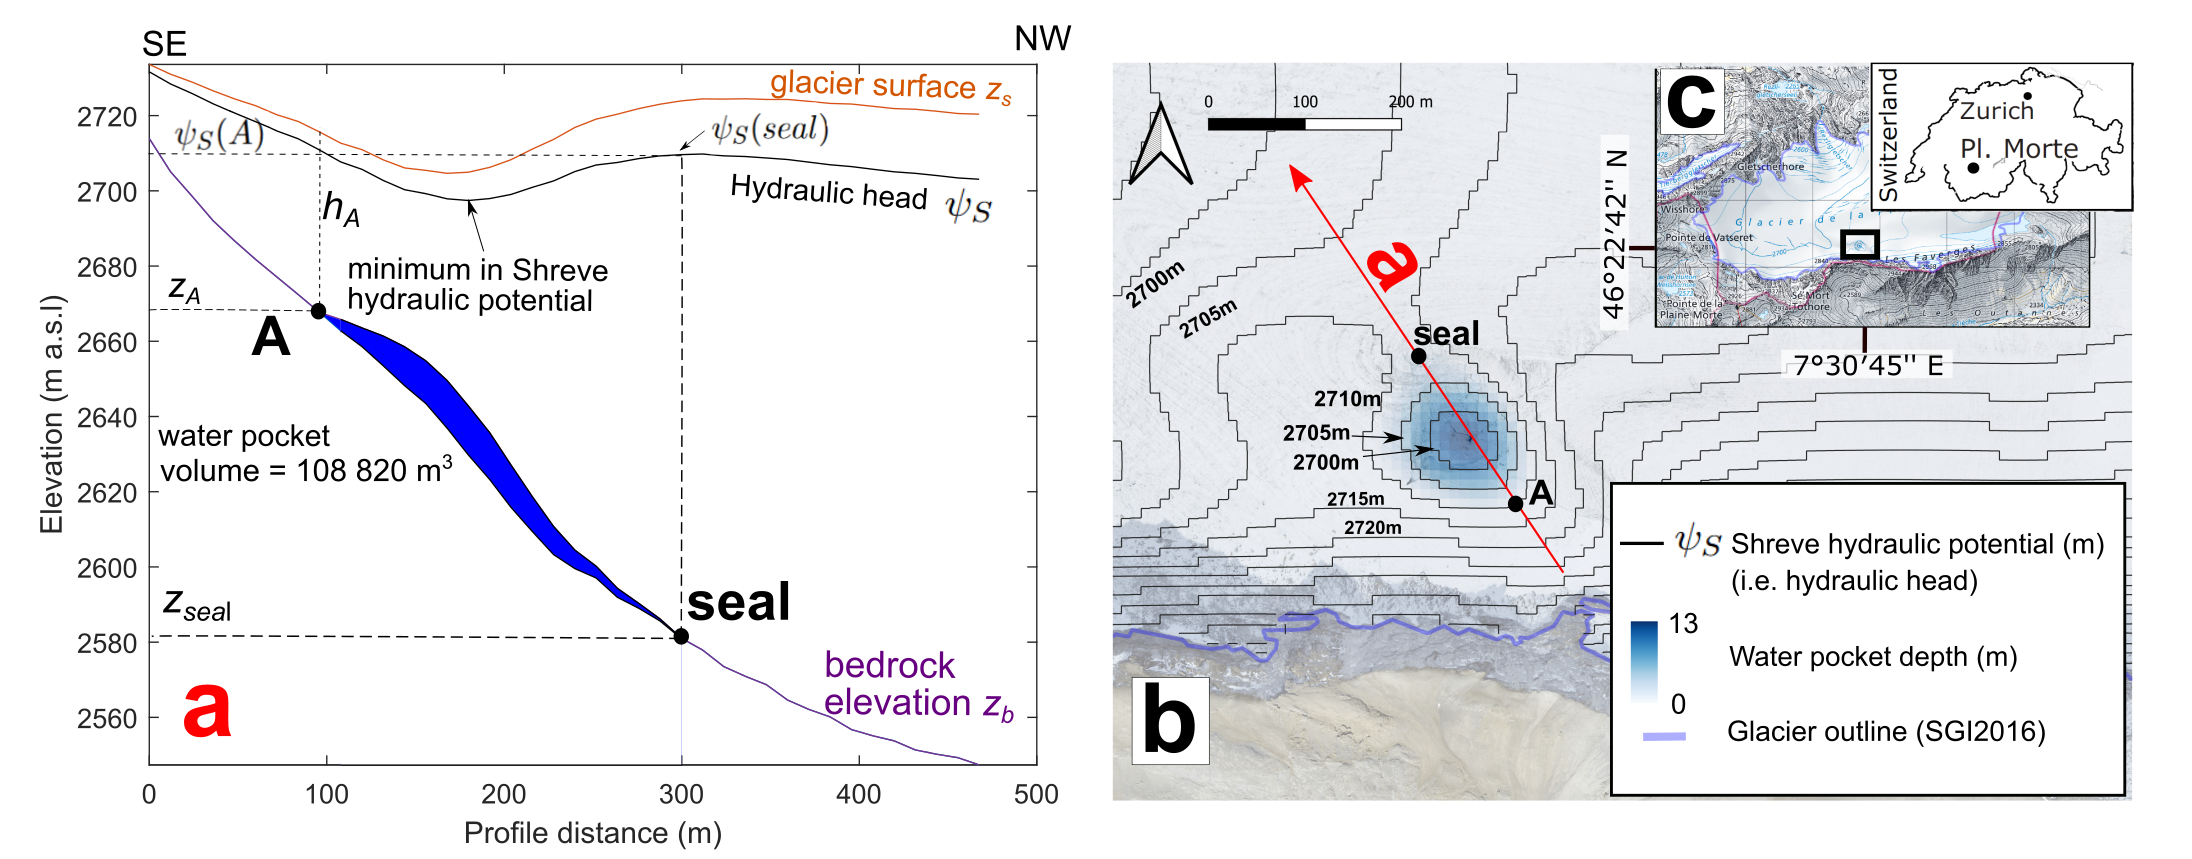
\includegraphics[width=1\linewidth]{chapters/chapter_WPOFs/PlaineMorte_WP_fig.png}
    \caption{a) Example of the cross section of a hypothetical water pocket caused by a hydraulic barrier at Glacier de la Plaine Morte (Switzerland). $z_s$, $z_b$ and $\psi_S$ are the surface elevation, the bedrock elevation and the hydraulic head, respectively, along the profile (red arrow) shown in panel b). ``A'' is the highest point of the water pocket before its rupture, in turn controlled by the hydraulic head at the seal. b) Orthophoto of Glacier de la Plaine Morte from the Federal Office of Topography (swisstopo) with the contour lines of $\psi_S$ in black and the water pocket depth in blue. The glacier outline is from the SGI2016 \citep{Linsbauer&al2021}. c) Topographic map from the Federal Office of Topography (swisstopo) and location of Glacier de la Plaine Morte in Switzerland.}
    \label{fig:plainemorteWP}
\end{figure*}


\subsection{ Water-filled crevasses}
%Difference with the thermal barrier case is that here the water reservoir already exists. In the thermal barrier case the water pocket geometry is controled by water pressure

A mechanism that could produce WPOF-type events is the emptying of water-filled crevasses in both temperate and polythermal ice. We argue that water-filled crevasses can be classified as water pockets when they are either fully englacial (see left water-filled crevasse in Fig.~\ref{fig:general_concept}) or relatively narrow at their top, making them more similar to englacial water bodies than to supraglacial ones (see middle water-filled crevasse in Fig.~\ref{fig:general_concept}). The water pocket rupture could be caused by hydrofracturing through the ice because of the water pressure \citep[e.g.][]{Benn&al2009,Scambos&al2009}, thus connecting the water-filled crevasse to the main drainage system and resulting in a progressive enlargement of the subglacial channel, and eventual flooding (see also Section~\ref{sec:hydraulic_barrier}). 

In temperate ice, water-filled crevasses are not common because they are typically well connected to the englacial drainage network and therefore cannot retain water \citep{Fountain&Walder1998}. Water can vertically penetrate through the entire ice column \citep{Weertman1973,VanderVeen1998} because the water density is higher than the ice density and because the water pressure can overcome the cryostatic pressure (hydrofracturing), in turn allowing water in crevasses to reach the glacier bed \citep{VanderVeen2007,Benn&al2009}. In 1920, a WPOF from water-filled crevasses was observed at the snout of Mellichgletscher \citep{Mercanton1921}. The WPOF at Tête Rousse in 1892 was explained by the formation of a supraglacial lake during a negative mass balance anomaly, and by the burial and isolation of this lake from the surface during the following years of positive mass balance \citep{Vincent&al2010b}. Although in that case the reservoir had developed from a supraglacial lake, the rupture mechanisms might have been similar to water-filled crevasses being isolated from the glacier surface. In 1904, a 22,000\,m$^3$ water-filled crevasse was artificially drained at Tête Rousse \citep{Vincent&al2010b}.

In cold ice, water-filled cavities can originate from the ice dynamic closure of supra-/englacial water channels or water-filled crevasses, both associated with the decrease in surface melt and water flow at the end of the melt season. Such a cut-and-closure mechanism is well documented and recognized in the literature \citep[e.g.][]{Gulley&al2009,Irvine&al2011} and is supported by numerical modelling \citep{Jarosch&Gudmundsson2012}. Water-filled crevasses can also propagate into cold ice by hydrofracturing \citep[e.g.][]{Benn&al2009,Scambos&al2009}. In the Swiss Alps, \cite{Haefeli&Brentani1955} observed an isolated water-filled crevasse of at least several hundred cubic meters in cold ice (-2°C) at Jungfraujoch (3467 \,m a.s.l., Bernese Oberland) in the 1950s. The authors attributed the origin of this water to melt water from the surface. \cite{Fisher1963} found a 100\,m$^3$ water-filled cavity in the cold ice of Breithorn peak (Valais) at 4000\,m a.s.l. \cite{Paterson&Savage1970} discovered a pressurized and isolated water-filled cavity (of unmeasured volume) at a depth of 9\,m in cold ice while drilling in Athabasca Glacier (Canada). Note that none of the water-filled reservoirs mentioned above have known outbursts, and that their volumes are relatively small. However, they illustrate the potential of englacial water storage in alpine cold ice. \cite{Vincent&al2015} suggested that the water pocket at Glacier de Tête Rousse (France) discovered in 2010 (that did not cause an outburst) was connected with another, smaller water reservoir located upglacier, that was in fact a water-filled crevasse. 
In summer 2022, the partial break-off of Ghiacciaio della Marmolada (Italy) resulted in a catastrophic ice avalanche that claimed the lives of eleven climbers. \cite{Bondesan&Roberto2023} as well as \cite{Chiarle&al2023} suggest that the glacier break-off was caused by high water pressure in a water-filled crevasse above a steep bedrock slope, and that the water-filled crevasse was presumably disconnected from the en-/subglacial drainage system due to cold ice (there are observations of water flowing out of the water-filled crevasses at the glacier surface before the detachment). The melt water volume produced in the catchment of the crevasse during seven weeks of abnormally high air temperature before the event was estimated to 11'000\,m$^3$ \citep{Bondesan&Roberto2023}. Similar to Ghiacciaio della Marmolada, the avalanching of Ghiacciaio glacier (Italy) that occurred in 1989 was also related to a water-filled crevasse prior to the collapse \citep{Dutto&al1991,Chiarle&al2023}. Albeit the Marmolada and Coolidge events might rather be categorized as ice avalanche rather than WPOFs, the englacial water accumulation preceding the partial glacier break-off stand exemplary for the potential of water storage in water-filled crevasses of cold or polythermal alpine glaciers. Cold ice acts as a thermal barrier by preventing water to flow. Note that for the water pocket formation mechanism presented in this section, the cavity (i.e.\ the crevasse) is already existing and filled with water after its formation. This differs from the mechanism presented in the next section, also related to polythermal conditions but called thermal barrier, where the cavity formation is initiated by water pressure exceeding the ice overburden pressure. 


\subsection{ Thermal barrier}
\label{sec:thermal_barrier}

We use the term "thermal barrier" to describe the water pocket formation mechanism in which a trapped subglacial water reservoir develops beneath the cold-temperate transition surface (CTS) of a polythermal glacier \citep[Fig.~\ref{fig:WPthermo}; see][for a review on the hydrology of polythermal glaciers]{Irvine&al2011}. At the early stage of water pocket formation, initial voids are not necessary, just some connection to the en-/subglacial drainage network upstream of the thermal barrier. Then, the growth of the water reservoir is controlled by ice creep vs. flotation due to high water pressure. Water pressure is in turn controlled by the slope of the bedrock upstream the water pocket and the water input \citep{Vincent&al2015}. If the upstream bedrock slope is steep and the water pressure higher than the ice pressure, the cavity will grow. This growth will continue until the ice dam is eventually broken or in hydrostatic equilibrium. The reservoir rupture that leads to the outburst flood may happen when the water pressure exceeds the ice overburden pressure at the glacier bed (similar to jökulhlaups, \cite{Bjornsson2010}), or when the ice temperature reaches the pressure melting point, allowing the water to run off subglacially by channel enlargement \citep[e.g.][]{Vincent&al2010b}.  

The best documented example for a water pocket formation and filing mechanism caused by thermal barrier is the one discovered in 2010 at Glacier de Tête Rousse at 3180\,m a.s.l. \citep{Vincent&al2012,Gilbert&al2012,Vincent&al2015}. In the Tête Rousse case, the particular topoclimatic factors (large snow accumulation at the top due to avalanches, relatively low accumulation at the tongue and a mean annual air temperature of around -3°C) associated with the glacier's small size and low slope caused a cold-based, firn-free "plug" at the glacier tongue, and firn-insulated temperate ice in the accumulation zone \citep{Gilbert&al2012}. In the firn-free area, the melt water runs off superficially, thus preventing any heat transfer into the ice by refreezing and latent heat release. In addition, the very low ice flow velocities of the glacier prevent the advection of temperate ice downstream or significant strain heating. This combination of factors was suggested to have caused the ice to be cold at such low elevations, resulting in the development of a water pocket over a period of about forty years \citep{Gilbert&al2012}. 

This relatively long persistence of a water pocket is in strong contrast to what is suggested by the analysis of WPOF events in the Swiss Alps compiled in our inventory (see Section~\ref{sec:inventary}) and to two of the other proposed WPOF formation and outburst mechanisms (temporary blockage of subglacial channels and hydraulic barriers). Although the thermal barrier mechanism seems to be a particularly good explanation for water pocket formation in general, there is no direct evidence for this type of mechanism in our updated WPOF inventory for the Swiss Alps. This could also be because they may rarely lead to a flood event and remain thus unreported. 

Assessing the likelihood for the thermal barrier mechanism to cause WPOFs in a given region would require knowledge about the englacial temperature distribution in that region. On a regional scale, however, reliable data about the spatial distribution of englacial temperatures is mostly lacking, making any assessment for the disposition of WPOFs caused by thermal barrier difficult. \cite{Huss&Fischer2016} modeled englacial temperatures for very small glaciers (<\,0.5\,km$^2$) in Switzerland, but their model outputs lack of comprehensive validation data which would be needed for a sound assessment of WPOF likelihood due to thermal barrier. By consequence, there is very little knowledge about the occurrence or likelihood of climatic and glacio-geomorphic conditions favorable for the formation of water pockets by thermal barrier as well as about the frequency of WPOFs caused by thermal barrier. This type of WPOF is of interest, however, as the potential flood magnitude is large due to subglacial water accumulation possibly occurring over long periods of time.


\begin{figure*}
    \centering
    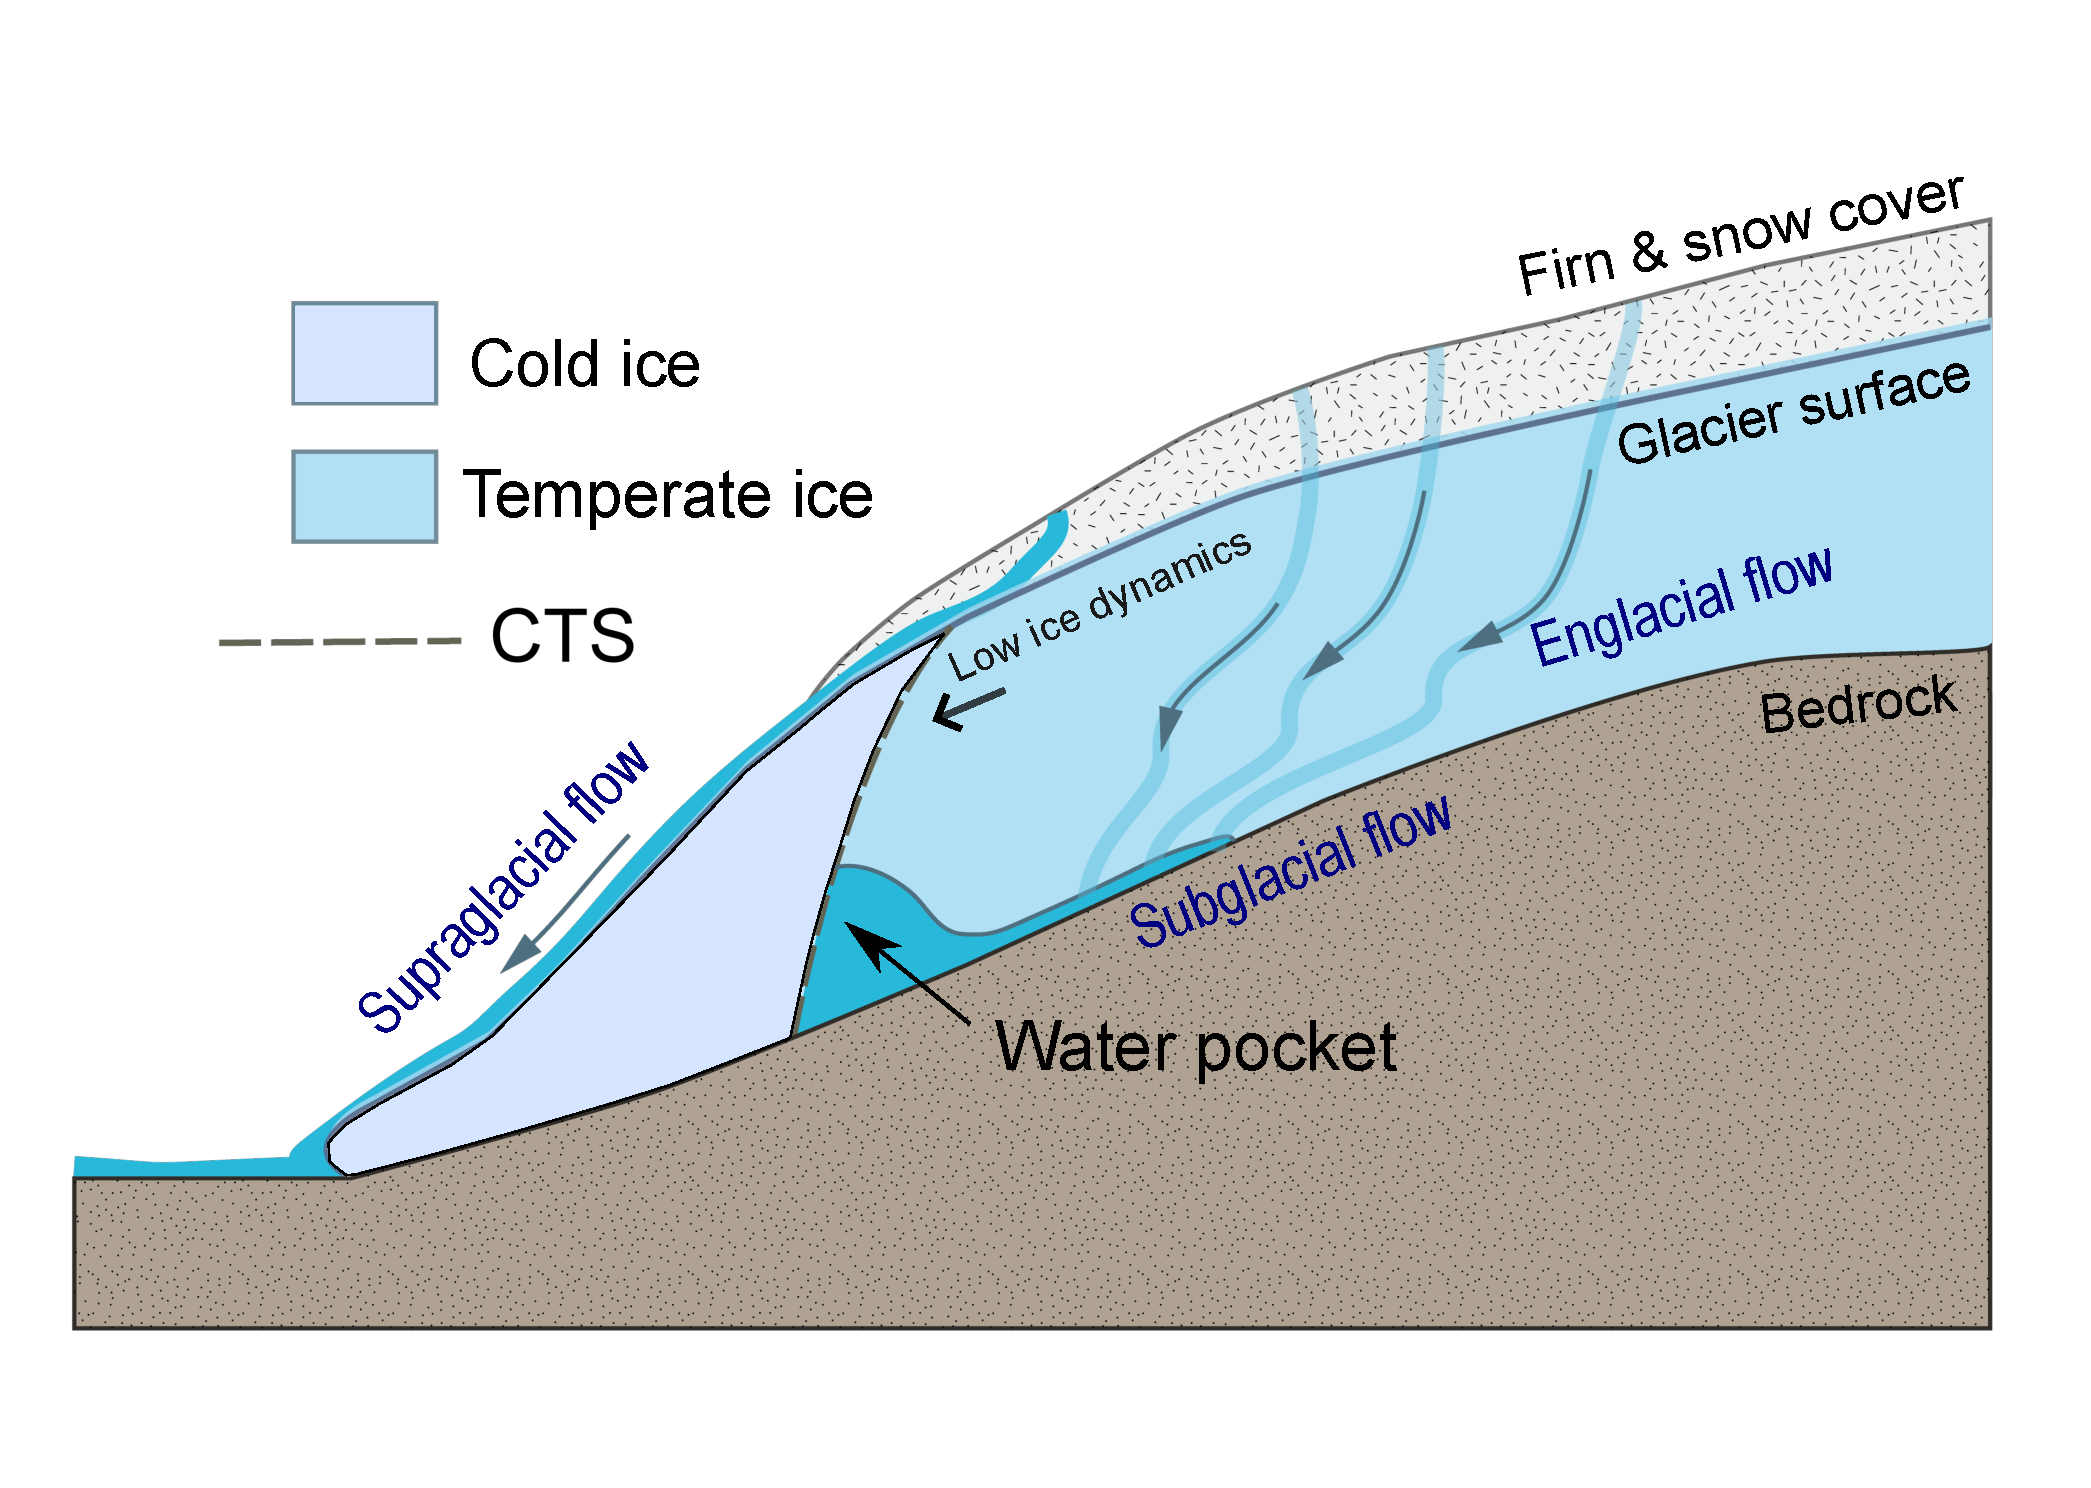
\includegraphics[width=0.7\textwidth]{chapters/chapter_WPOFs/thermal_barrier.pdf}
    \caption{Schematic of a water pocket caused by a thermal barrier. "CTS" stands for cold-temperate transition surface. Below the firn and snow cover, the temperate ice is isolated from the penetration of cold air temperatures into the ice through conductive cooling, and the percolation and refreezing of water in the firn releases heat. Over the firn-free area, melt water runs off superficially, thus not transferring any heat into the ice. Due to the absence of firn and snow, cold air temperatures lead to conductive cooling of the ice. The geometry of the water pocket is driven by the ice and water pressure, the latter is controlled by the slope of the bedrock and the upslope water input.}
    \label{fig:WPthermo}
\end{figure*}


\section{ Discussion}

\subsection{ Implications of the meteorological analyses on the formation and the rupture of water pockets}

The results of the meteorological analysis (Section~\ref{sec:envelop_meteo}) suggest that the formation and rupture of water pockets in temperate glaciers is most often linked to short-term processes (i.e.\ processes that take a maximum of a few days), and more specifically to meltwater input. The rupture of water pockets caused by precipitation input, instead, seems to play only a secondary role, since WPOFs do not always occur together with or after intense precipitation. Nevertheless, in individual cases, precipitation might play a role in triggering WPOFs by saturating and destabilizing the englacial and subglacial drainage network \citep[e.g.][]{Warburton&Fenn1994}. The timing and intensity of the precipitation event might be more important for the triggering of WPOFs than the total water amount. This is because fast water input can produce high water pressure, especially when the glacier's drainage capacity is limited \citep[e.g.][]{Warburton&Fenn1994,Sugiyama&Gudmundsson2004}. Since the sub-daily precipitation intensity is not known for most of the WPOF events in our inventory, however, it is difficult to further investigate this relationship.

The fact that the formation processes of water pockets in the Swiss Alps typically occur within a few days suggests that the water predominantly fills pre-existing cavities. Indeed, the process of opening glacial cavities is relatively slow \citep[e.g.][]{Vincent&al2015}, and is unlikely to occur within the time frame of a few days. Water pockets formed by short-term processes such as temporary blockages (see Sec.~\ref{sec:subglacialblocking}) are likely part of an active en-/subglacial drainage system, which we think is the most common case in temperate glaciers. Conversely, water pockets isolated from the drainage system may accumulate water over longer time spans, and are thus more likely to occur under particular climatic and glacio-geomorphic conditions, such as the ones prevailing at the polythermal Glacier de Tête Rousse (see Section~\ref{sec:thermal_barrier}).


\subsection{ Relation between water pocket outburst floods volume and peak discharge}
\label{sec:prediction}

Empirical relations simply considering lake volume ($V$) have proven useful for estimating peak discharges ($Q_{\rm{max}}$) of GLOFs. For instance, \citet{Clague&Mathews1973} proposed the relationship $Q_{\rm{max}} = 75(V/10^6)^{0.67}$ ($V$ in m$^3$ and $Q$ in m$^3$\,s$^{-1}$) based on their study of 10 GLOFs caused by progressive enlargement of ice channels, while \citet{Haeberli1983} suggested that a rough estimate of $Q_{\rm{max}}$ can be obtained by simply dividing the total lake volume $V$ by the characteristic time $t$ over which a flood occurs (i.e.\ $ Q_{\rm{max}} = V /t$, with $t$ being typically in the order of 800 to 2500\,s in \cite{Haeberli1983}). One might question whether analogous relationships could be formulated for WPOFs as well. Importantly, a notable distinction lies in the estimation of the water pocket volume, which can only be achieved after the WPOF event and which is equal to the flood volume ($V_{\rm{flood}}$), contrasting with GLOFs, for which lake volume ($V$) is typically estimated before the outburst. In our updated WPOF inventory, 11 entries contain information about both total flood volume $V_{\rm{flood}}$ (in m$^3$) and peak discharge of the flood $Q_{\rm{max}}$ (in m$^3$\,s$^{-1}$). The two quantities are plotted against each other in Fig.~\ref{fig:vflood_qmax}, together with the two empirical relations used for GLOFs by \citet{Clague&Mathews1973} and \citet{Haeberli1983}. As shown in Fig.~\ref{fig:vflood_qmax}, the scatter between $V_{\rm{flood}}$ and $Q_{\rm{max}}$ is large for WPOFs in Switzerland with available data, and there is moderate agreement with empirical relations established for GLOFs (coefficient of determination $r^2$ = 0.58 for the relation by \cite{Clague&Mathews1973}, and $r^2$ = 0.61 for the one by \cite{Haeberli1983} when fitting $t$ = 4600\,s to our observations). Note that $t$ acts as a scaling factor that determines the magnitude of $Q_{\rm{max}}$ for a given $V$. Changing the value of $t$ simply shifts the linear relationship along the $Q_{\rm{max}}$ axis but does not change the slope of the line. Available data on $Q_{\rm{max}}$ and $V_{\rm{flood}}$ in our inventory are not calculated using the same method. $Q_{\rm{max}}$ was either modelled or gauged at various time intervals and/or at various distance from the glacier portal (the further downstream the gauging station, the more dampened the discharge signal), and $V$ was calculated either with or without considering the baseflow (see also Section~\ref{Sec:Spatio_temporal}). The large scatter observed in Fig. \ref{fig:vflood_qmax} between $Q_{\rm{max}}$ and $V_{\rm{flood}}$ can be attributed to several local factors influencing the hydrograph of each flood event. Consequently, floods with similar total volumes may exhibit varying peak discharges. Among these factors, the distance between the flood origin and the gauging station for $Q_{\rm{max}}$ might be one of the most important. Typically, $Q_{\rm{max}}$ decreases downstream for any given flood. Additionally, the diverse range of mechanisms involved in water pocket ruptures (as detailed in Section \ref{sec:mechanisms}) likely contributes to this significant scatter. We conclude that with our dataset, no robust relation can be established between WPOF volumes and peak discharge. It is worth noting that even if a more robust relationship could be established, the lack of knowledge regarding the water pocket volume before the outburst diminishes the relevance of the relationship between flood volume and peak discharge for hazard mitigation.


\begin{figure}
    \centering
    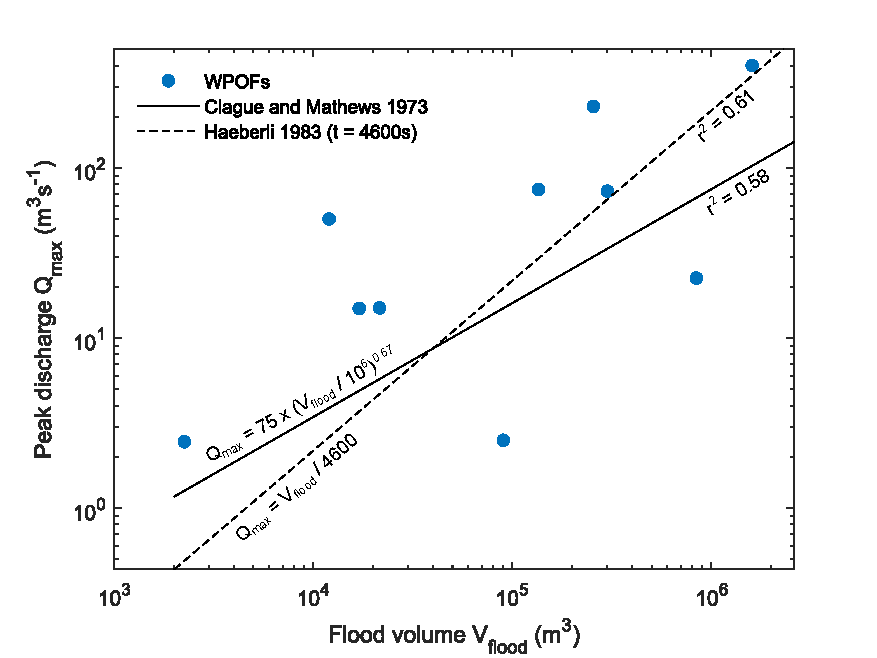
\includegraphics[width=0.8\linewidth]{chapters/chapter_WPOFs/Qmax_Vflood_scaling.pdf}
    \caption{Relation between flood volume ($V_{\rm{flood}}$) and peak discharge ($Q_{\rm{max}}$) for WPOFs in the Swiss Alps for which these data are available (n\,=\,11). The solid line represents the relationship between GLOFs' volume and peak discharge by \cite{Clague&Mathews1973}. The dashed line represents the relationship between GLOFs' volume and peak discharge by \cite{Haeberli1983} using $t$\,=\,4600\,s.}
    \label{fig:vflood_qmax}
\end{figure}


\subsection{ Perspectives for further research}

% Lack of Direct Observations
The absence of direct observations of water pockets prior to and during outburst floods significantly limits our understanding of this phenomenon. By consequence, it is important for further research to prioritize the detection and monitoring of water pockets. For instance, while the water pocket at Glacier de Tête Rousse has been extensively studied (see Section~\ref{sec:thermal_barrier}), it represents only one of the four potential formation mechanisms proposed in this study, and, to our knowledge, there are no other direct observations of such phenomena. 

% Ground-Based Detection Methods
Detection of water bodies within glaciers can be achieved through geophysical techniques such as ground-penetrating radar \citep[e.g.][]{Vincent&al2012,Church&al2021}, surface nuclear magnetic resonance \citep[e.g.][]{Legchenko&2014,Garambois&al2016}, and seismic methods \citep[e.g.][]{Horgan&al2012,Guillemot&al2024}. However, these methods typically entail substantial logistics and field effort, making them unsuitable for deployment across the entire glacier, but rather applicable to areas covering a few thousands square meters at most. Consequently, prior knowledge of potential water pocket locations is often necessary before deploying these methods \citep[e.g. the use of surface nucleid magnetic resonance following ground-penetrating radar analysis, as in][]{Vincent&al2012}. 

% Detection from Space
Detection of water pockets forming due to hydraulic and thermal barriers could be observed through changes in surface elevation. As these two mechanisms involve cavity growth within the glacier, changes in surface elevation during filling (i.e.\ uplift) and drainage (i.e.\ lowering) phases could be detected using remote sensing techniques such as differencing of consecutive digital elevation models (DEMs) or Interferometric Synthetic Aperture Radar (InSAR).

For instance, \cite{livingstone&al2019} detected drainage of three subglacial lakes in Greenland with minimal volumes of 3.5–13$\,\times$\,10$^6$\,m$^3$ using satellite stereo-images and DEM differencing (note that although the authors use the term subglacial lake, we would call them water pockets in this study since they were not formed by geothermal activity). Although achieving the required temporal, horizontal, and in particular vertical spatial resolution for accurate detection of small water pockets at the regional scale may be challenging, there is potential for obtaining high-resolution DEMs at the glacier scale, e.g. by using unmanned aerial vehicles (UAV) \citep[see][for UAV applications in glaciology]{Bhardwaj&al2016,Groos&al2022}.

\cite{Capps&al2010} analysed patterns of eight InSAR-derived interferograms that indicate the subsidence of the glacier surface over three water pockets at Brady Glacier (Alaska, USA). The detected change in water volume ranged from 22'000 to 243'000\,m$^3$. The authors could not definitively assess the potential for a sudden water pocket drainage because the coherent radar data were too far spaced in time. Nevertheless, they claim that deploying this technique successfully in other glacierized alpine regions could enable the recognition and quantification of water pockets (named subglacial lakes in their study) prior to hazardous outburst floods. However, the difference in acquisition time between two images needs to be adequate for applying this technique to water pockets detection. Acquisition time difference needs to be short enough to prevent decorrelation in the interferograms that is due to glacier motion, but large enough to capture the small changes in glacier surface elevation due to water pocket growth. 

The presence of snow at the glacier surface may limit the remote detection of supraglacial terrain features that point to water pocket growth or emptying because snow redistribution by wind usually smoothes out the glacier surface topography. For instance, at Glacier de Tête Rousse, DEM differencing fails to detect the depression caused by artificial water pocket drainage due to significant snow accumulation \citep{Gagliardini&al2011}.

% Importance of Thermal Regime Characterization
Water pockets formed due to thermal barriers might pose the highest flood potential \citep{Vincent&al2010b}. Therefore, characterizing a glacier's thermal regime is crucial to identify potential water pocket locations at the cold-temperate transition surface. By accurately modelling the thermal regime of glaciers at the regional scale (e.g. the Alps), one could highlight potential locations that have a favorable disposition for water pockets to form. In recent years, research on the thermal characterization of alpine glaciers has progressed from simplistic 1D modeling \citep[e.g.][]{Gilbert&al2014,Huss&Fischer2016} to more complex three-dimensional full-Stokes models \citep[e.g.][]{Gilbert&al2015}. However, in-situ temperature measurements for validation are scarce \citep[e.g.][for the Swiss Alps]{Luthi&Funk2001,Huss&Fischer2016}, and the high computational demands of these physically-based models currently prevent their applicability at the regional scale.

% Water Balance Calculation
Understanding water pocket formation requires assessing a glacier's capacity to store water englacially and subglacially. Calculating the water balance at the glacier scale, i.e. the ratio of input and output of water over time, allows the quantification and duration of stored water volume \citep[see][for a review on glacier storage concepts]{Jansson&al2003}. While water output can often be well constrained by discharge measurements at proglacial streams, water input is commonly estimated with limited in-situ measurements through modeling of snowmelt, ice melt and rain \citep[e.g.][]{Hock2005}. Moreover, the phase changes that are evaporation, condensation, sublimation and deposition between the input and output of water are difficult to constrain. Consequently, the inherent uncertainties associated with water balance calculations may hinder accurate short-term water storage quantification, particularly for short-term mechanisms such as temporary subglacial channel blockages. Nevertheless, higher temporal resolution measurements of the inputs and outputs to glacial stream flow could offer valuable insights into these processes \citep[e.g.][]{Muller&al2024b}.


\section{ Conclusion}

In this study, we reviewed the existing literature on alpine glacial water pockets to propose a clear definition of all phenomena that can, in our opinion, be summarized under this term. In addition, we extended, updated and analysed a pre-existing inventory of water pocket outburst floods (WPOFs) in Switzerland. We found that the term "water pocket" has frequently been employed by default to describe unknown subsurface water reservoirs at the origin of unexplained glacial outburst floods. We defined an alpine glacial water pocket as an englacial or subglacial water-filled cavity with a typical volume larger than 1000\,m$^3$, and explicitly excluded subglacial lakes formed by geothermal heat. In our inventory, we compiled information on 91 WPOFs for 37 glaciers, including 20 glaciers with repetitive WPOFs. Direct observations of the en-/subglacial water reservoir are only documented for three WPOFs. In general, we suspect that a significant portion of WPOFs goes unnoticed and is therefore missing in our inventory. This can be explained by the lack of observations and the difficulty in detecting flood signals related to particularly smaller WPOFs at gauging stations positioned far downstream of the glacier snout. 

Analysis of reported WPOFs in the Swiss Alps since 1900 to the present reveals no significant temporal trend in their occurrence. Detecting such trends is challenging due to suspected spatial and temporal observational biases. The majority of WPOFs occurs between June and September, indicating the importance of water input from snowmelt, ice melt or rain for the (re-)formation and rupture of water pockets. Among the 32 WPOFs for which gridded daily meteorological data was available, our analysis revealed anomalously high temperatures during several (typically one or two) days prior to the event. Additionally, strong to heavy precipitation (>\,10\,mm during the event day) coincides with a quarter of these 32 WPOFs. This indicates that the majority of water pockets recorded in our inventory likely formed in pre-existing voids within a few days only due to significant water input from melting and/or intense precipitation. The resulting high influx of meltwater and/or precipitation into the en-/subglacial drainage system of temperate glaciers is likely to trigger drainage instability leading to the water pocket rupture and thus the outburst. Conversely, water pockets that are isolated from the drainage system and accumulate water over longer periods (years to decades) are more likely to form in polythermal glaciers. This is particularly well demonstrated for the water pocket detected in Glacier de Tête Rousse in 2010 which seems to have developed over a period of 40 years. Our analysis of the reported WPOFs in the Swiss Alps also suggests that glacier-wide glacio-geomorphic variables are likely not sufficient to identify glaciers that are susceptible to WPOFs. Indeed, water pocket formation is likely controlled by smaller-scale and very local topographic features, but our inventory lacks precise data on water pocket locations, hence hindering further analysis at higher spatial resolution.

Based on our WPOF inventory for the Swiss Alps and a literature review, we propose four mechanisms responsible for the formation of water pockets in alpine glaciers: 1) temporary blockage of subglacial channels, 2) hydraulic barriers, 3) water-filled crevasses, and 4) thermal barrier. WPOFs caused by a temporary blockage occur when ice blocks collapse from the roof of a subglacial channel or a subglacial cavity, leading to blockage and water accumulation within the glacier, which can result in a sudden release of water when the ice dam breaks. This mechanism was found to be the most frequent in our WPOF inventory. WPOFs caused by a hydraulic barrier occur when water accumulates at the glacier bed in areas where there is a local minimum in the hydraulic potential, which is controlled by the ice surface and the bedrock geometry. The ice surrounding this minimum hydraulic potential acts as an ice dam, obstructing the flow of subglacial water and leading to the formation of a water pocket. The ice dam breaks when the water pressure exceeds the pressure of the overburden ice at the seal, leading to the emptying of the water pocket through the subglacial drainage network. WPOFs caused by water-filled crevasses occur when such crevasses are isolated from the main drainage system but eventually connect back by hydrofracturing through the ice, resulting in a progressive enlargement of the subglacial channel and leading to an outburst. Finally, WPOFs caused by thermal barrier occur when subglacial water is trapped at the cold-temperate transition surface of polythermal glaciers, eventually leading to outburst floods when the water pressure exceeds the ice overburden pressure or when the ice temperature reaches the pressure-melting point. This mechanism is well documented for Glacier de Tête Rousse in the French Alps, but could not be assigned to any of the WPOF glaciers included in our inventory for the Swiss Alps.

To further deepen our understanding of the mechanisms controlling water pocket formation and rupture, we encourage more field-based research. In particular, we propose observational techniques that aim at detecting and monitoring water pockets within alpine glaciers, since the lack of observations currently constitutes a crucial limitation in the understanding of WPOFs. The difficulty in detecting the exact locations of water pockets is the most limiting factor in this respect. We hope that our study will foster the interest in such endeavors.

\section{ Code and Data Availability}

The WPOF inventory described and analysed in Section~\ref{sec:inventary} can be accessed via \url{https://github.com/christopheogier/WPOFs_CH.git} (Note that this link will be replaced by a DOI handle in the event of this work being accepted for publication). The distributed map of the theoretical subglacial water pocket volumes for all Swiss glaciers (see Section~\ref{sec:hydraulic_barrier}) is available through ETH Zurich's Research Collection, DOI:\,\texttt{10.3929/ethz-b-000667509}. The Julia programming language package WhereTheWaterFlows.jl is accessible at \url{https://github.com/mauro3/WhereTheWaterFlows.jl}. The version used here is v0.8.1 and archived at \url{https://doi.org/10.5281/zenodo.8061564}.\\

\section{ Acknowledgements} 

This project was financially supported by the Swiss National Science Foundation (grant nr. 212061). The contributions by M. Fischer were funded by the University of Bern, Switzerland. The contributions by M. Thibert, A. Gilbert, C. Vincent and O. Gagliardini were partially funded by 
the Ministère de la Transition écologique et de la Cohésion des territoires (French ministry for Ecological Transition and Territorial Cohesion) through 
its PAPROG program. The authors thank Dorde Masovic for his work on the Figures~\ref{fig:general_concept},~\ref{fig:IceBlockage}, and~\ref{fig:WPthermo}. The authors thank Felix Altrock, Sarah Lanz, Claudio Steffen, Flavia Zimmermann, Eric Bardou, Daniel Devanthery, Raphaël Mayoraz, Martin Proksch and Nils Hählen for their contributions to the WPOFs inventory. The authors thank Alpiq SA for providing streamflow discharge data.




